\documentclass{beamer}
\usepackage[english]{babel}
\usepackage{amsmath,amssymb,graphicx,latexsym,tabularx,calc,capt-of,xcolor,ifthen,theorem}

%%%%%%%%%% Start TeXmacs macros
\newcommand{\assign}{:=}
\newcommand{\infixand}{\text{ and }}
\newcommand{\mathd}{\mathrm{d}}
\newcommand{\nocomma}{}
\newcommand{\qed}{$\Box$}
\newcommand{\tmcolor}[2]{{\color{#1}{#2}}}
\newcommand{\tmmathbf}[1]{\ensuremath{\boldsymbol{#1}}}
\newcommand{\tmmisc}[1]{\thanks{\textit{Misc:} #1}}
\newcommand{\tmop}[1]{\ensuremath{\operatorname{#1}}}
\newcommand{\tmsamp}[1]{\textsf{#1}}
\newcommand{\tmtextbf}[1]{{\bfseries{#1}}}
\newcommand{\tmtextit}[1]{{\itshape{#1}}}
\newcommand{\tmverbatim}[1]{{\ttfamily{#1}}}
\newenvironment{proof}{\noindent\textbf{Proof\ }}{\hspace*{\fill}$\Box$\medskip}
\newtheorem{lemma}{Lemma}
{\theorembodyfont{\rmfamily}\newtheorem{remark}{Remark}}
\newtheorem{theorem}{Theorem}
\newcommand{\tmfloatcontents}{}
\newlength{\tmfloatwidth}
\newcommand{\tmfloat}[5]{
  \renewcommand{\tmfloatcontents}{#4}
  \setlength{\tmfloatwidth}{\widthof{\tmfloatcontents}+1in}
  \ifthenelse{\equal{#2}{small}}
    {\setlength{\tmfloatwidth}{0.45\linewidth}}
    {\setlength{\tmfloatwidth}{\linewidth}}
  \begin{minipage}[#1]{\tmfloatwidth}
    \begin{center}
      \tmfloatcontents
      \captionof{#3}{#5}
    \end{center}
  \end{minipage}}
%%%%%%%%%% End TeXmacs macros

% \#Partial Derivative symbol

\newcommand{\pdv}[2]{\frac{\partial #1}{\partial #2}}
\newcommand{\pdv*}[3]{\frac{\partial^{#1} #2}{\partial #3^{#1}}}
% \#Ordinary derivative symbol

\newcommand{\dv}[2]{\frac{\mathd #1}{\mathd #2}}
\newcommand{\dv*}[3]{{\frac{\ensuremath{d^{#1} #2}}{d \ensuremath{#3^{#1}}}}}
% \#Bold symbols - Start

\newcommand{\bC}{\ensuremath{\tmmathbf{C}}}
\newcommand{\bd}{\ensuremath{\tmmathbf{d}}}
\newcommand{\bD}{\ensuremath{\tmmathbf{D}}}
\newcommand{\be}{\ensuremath{\tmmathbf{e}}}
\newcommand{\bE}{\ensuremath{\tmmathbf{E}}}
\newcommand{\bof}{\ensuremath{\tmmathbf{f}}}
\newcommand{\bF}{\ensuremath{\tmmathbf{F}}}
\newcommand{\bg}{\ensuremath{\tmmathbf{g}}}
\newcommand{\bG}{\ensuremath{\tmmathbf{G}}}
\newcommand{\bl}{\ensuremath{\tmmathbf{l}}}
\newcommand{\bM}{\ensuremath{\tmmathbf{M}}}
\newcommand{\bp}{\ensuremath{\tmmathbf{p}}}
\newcommand{\bP}{\ensuremath{\tmmathbf{P}}}
\newcommand{\bq}{\ensuremath{\tmmathbf{q}}}
\newcommand{\bS}{\ensuremath{\tmmathbf{S}}}
\newcommand{\br}{\ensuremath{\tmmathbf{r}}}
\newcommand{\bu}{\ensuremath{\tmmathbf{u}}}
\newcommand{\bv}{\ensuremath{\tmmathbf{v}}}
\newcommand{\bw}{\tmmathbf{u}}
\newcommand{\bx}{\ensuremath{\tmmathbf{x}}}
% \#Bold symbols-end


\begin{document}

{\screens{\begin{frame}
  {\unrollgreyed{\title{Annual Thesis Committee (TC) meeting\tmmisc{Arpit
  Babbar}}
  
  \date{July 6, 2022}
  
  \maketitle}{\tmtextbf{Main developments}
  \begin{itemize}
    {\unrollgreyed{\item Extended Zhang-Shu's positivity limiter
    {\cite{Zhang2010b}} to Lax-Wendroff schemes to obtain a provably
    admissibility preserving Lax-Wendroff scheme}{\item Developed blending
    limiter of Hennemann Et Al {\cite{HENNEMANN2021109935}} for Lax-Wendroff
    schemes. Improved the lower order part of blending from first order finite
    volume method to second order MUSCL-Hancock method.}{\item Extended proof
    of admissibility of MUSCL-Hancock method by Berthon {\cite{Berthon2006}}
    to non-cell centred finite volume grids used by
    {\cite{HENNEMANN2021109935}}. Used a problem independent procedure to
    limit slope for admissibility.}{\item Made theoretical comparison of
    Lax-Wendroff and ADER schemes - proved equivalence for linear case with D2
    dissipation and \tmtextit{closeness} for non-linear case.}}
  \end{itemize}}{\tmtextbf{Structure of presentation}
  \begin{itemize}
    {\unroll{\item Review of Lax-Wendroff Flux Reconstruction with D2
    dissipation numerical flux.}{\item Brief introduction to the blending
    limiter of {\cite{HENNEMANN2021109935}}.}{\item Extending Zhang-Shu's
    limiter {\cite{Zhang2010b}} to Lax-Wendroff schemes.}{\item Admissibility
    preserving MUSCL-Hancock reconstruction on non-cell centred grids used by
    {\cite{HENNEMANN2021109935}}.}{\item Prove equivalence of ADER and LW-D2
    schemes with numerical verification, also recall instability issues noted
    in RKDG schemes by Xu Et Al in {\cite{Xu2019}}.}{\item Numerical results
    demonstrating admissibility preservation and accuracy improvement of
    limiting procedure.}{\item Summary and future plans}}
  \end{itemize}}}
  
  \ 
\end{frame}}{\begin{frame}
  \frametitle{Flux Reconstruction (FR) by Huynh {\cite{Huynh2007}}}
  
  {\unrollphantoms{\[ \large{u_t + f (u)_x = 0}
  \]}{\raisebox{-0.5\height}{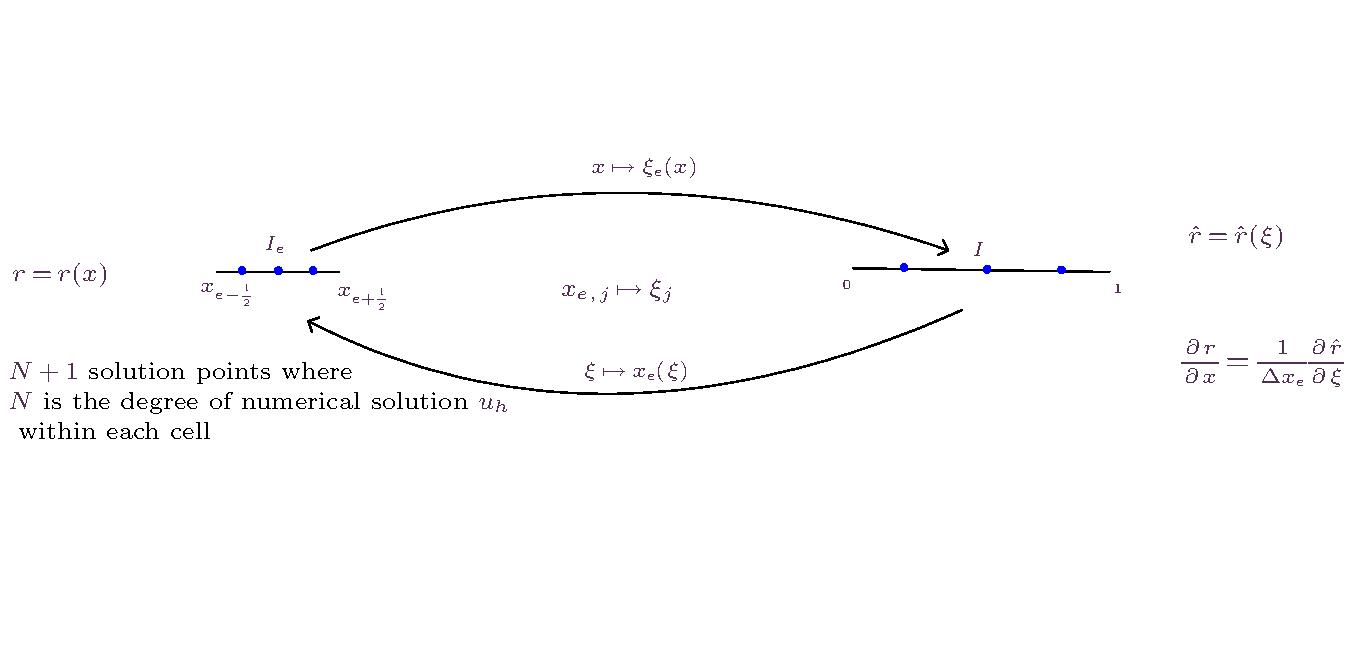
\includegraphics[width=22.8239210284665cm,height=11.0062639380821cm]{slides-1.pdf}}}}
\end{frame}}{\begin{frame}
  {\unroll{\frametitle{Flux Reconstruction (FR) by Huynh {\cite{Huynh2007}}}
  
  
  \[ \large{\begin{array}{c}
       \tmcolor{blue}{\dv{}{t} u_{e, i}} = - \pdv{f_h}{x} (x_{e, i}), \quad 1
       \leq i \leq N + 1.
     \end{array}} \]
  
  
  \
  
  \
  
  \resizebox{330pt}{250pt}{\includegraphics{slides-2.pdf}}\resizebox{330pt}{250pt}{\includegraphics{slides-3.pdf}}}}
\end{frame}}{\begin{frame}
  \frametitle{Flux Reconstruction (FR) by Huynh {\cite{Huynh2007}}}
  
  {\unroll{\raisebox{-0.5\height}{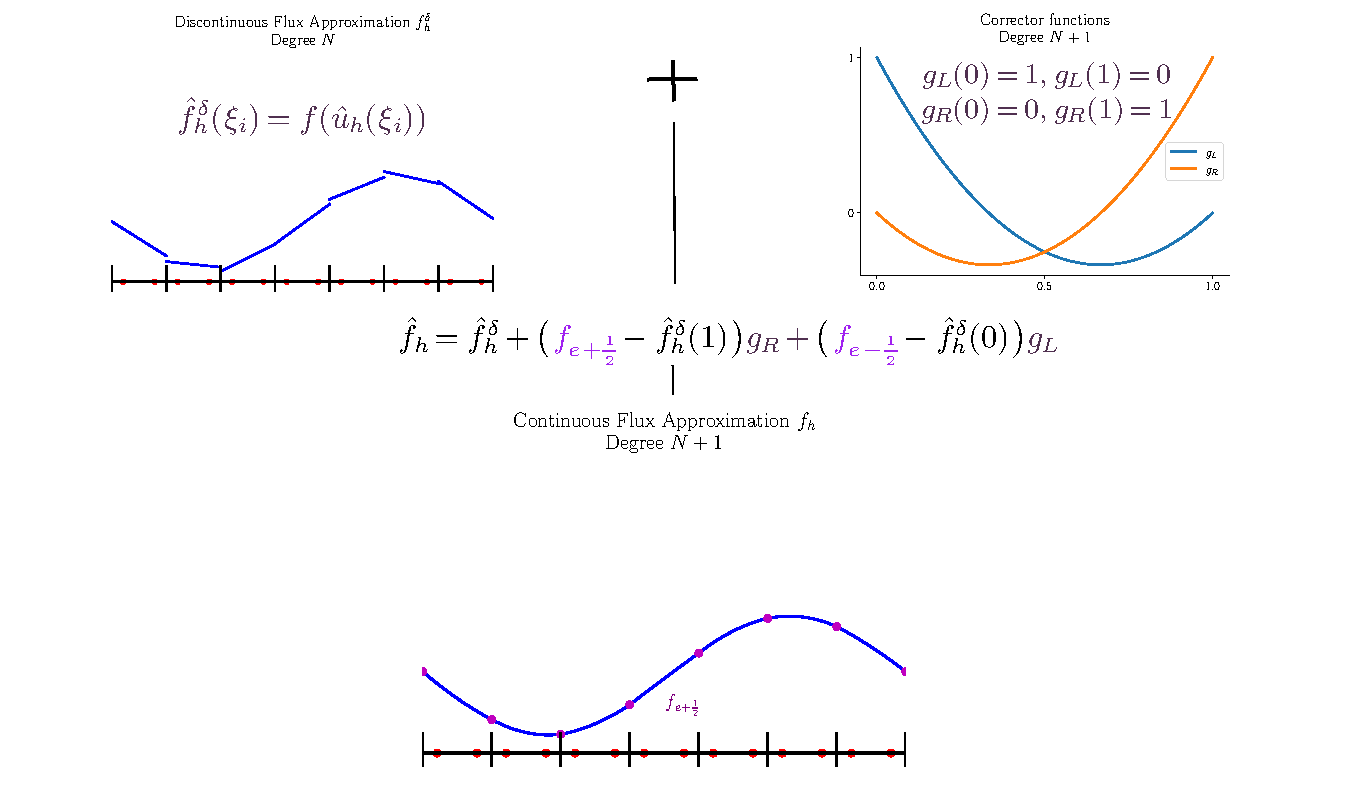
\includegraphics[width=22.8239210284665cm,height=13.3861996589269cm]{slides-4.pdf}}}}
\end{frame}}{\begin{frame}
  \frametitle{Lax-Wendroff Flux Reconstruction (LWFR) with D2 dissipation}
  
  {\unroll{\[ \begin{array}{c}
       \large{u^{n + 1} = u^n - tF^n_x},\\
       \text{where } F = f (u) + \frac{t}{2} (f (u))_t + \frac{t^2}{3!} f
       (u)_{tt} + \cdots + \frac{t^N}{(N + 1) !} \pdv*{N}{}{t} f (u)
     \end{array} \]}{To compute $F$, we use the approximate Lax-Wendroff
  procedure proposed by Zorio Et Al. {\cite{zorio_approximate_2017}}
  \[ \begin{array}{ccc}
       f (u)_t & \approx & \frac{f (u (x, t + t)) - f (u (x, t - t))}{2 t} + O
       (t^2)\\
       & \approx & \frac{f (u + t \tmcolor{blue}{u_t}) - f (u - t
       \tmcolor{blue}{u_t})}{2 t} + O (t^2),
     \end{array} \]
  and\tmcolor{blue}{ \tmcolor{blue}{\tmcolor{blue}{$\tmcolor{blue}{u_t = - f
  (u)_x}$}}}.}{This will give us a discontinuous flux polynomial
  $F_h^{\delta}$ which we will correct with Flux Reconstruction (FR) using
  numerical flux $F_{e + \frac{1}{2}}$ and denote corrected flux by $F_h$.}{In
  the past works, $F_{e + \frac{1}{2}}$ has been computed as
  \[ \begin{array}{c}
       F_{e + \frac{1}{2}} = (F_L, F_R, u_L, u_R),\\
       u_L = u_h (x_{e + 1 / 2}^-), \qquad u_R = u_h (x_{e + 1 / 2}^+) .
     \end{array} \]}{In \tmcolor{red}{cite}, we propose the
  \tmtextbf{Dissipation 2} flux
  \[ u_L = U_h (x_{e + 1 / 2}^-), \qquad u_R = U_h (x_{e + 1 / 2}^+), \]
  where
  \[ U_h = u + \frac{t}{2} u_t + \frac{t^2}{3!} u_{tt} + \cdots +
     \frac{t^N}{(N + 1) !} \pdv*{N}{u}{t} \approx \frac{1}{t} \int_{t^n}^{t^{n
     + 1}} u_h d t. \]}}
  
  \ 
\end{frame}}{\begin{frame}
  \frametitle{Conservation property of LWFR}
  
  {\unroll{\[ (u^e_j)^{n + 1} = (u_j^e)^n - \frac{t}{x_e}  \pdv{F_h}{\xi}
     (\xi_j), \qquad 1 \leq j \leq N + 1. \]}{For $\{ w_j \}_{j = 1}^{N + 1}$
  being the quadrature weights associated to solution points,
  \[ \sum_{j = 1}^{N + 1} w_j (u^e_j)^{n + 1} = \sum_{j = 1}^{N + 1} (u_j^e)^n
     - \frac{t}{x_e}  \sum_{j = 1}^{N + 1} w_j  \pdv{F_h}{\xi} (\xi_j), \]}{\[
  \Rightarrow \overline{u}_e^{n + 1} = \overline{u}_e^n - \frac{t}{x_e} \left[
     F_{e + \frac{1}{2}} - F_{e - \frac{1}{2}} \right] \]}{We call this the
  \tmcolor{red}{conservation property}.}}
  
  \ 
\end{frame}}{\begin{frame}
  \frametitle{Blending limiter}
  
  {\unrollcompressed{Here we apply the Blending limiter of \ of Hennemann Et
  Al. {\cite{HENNEMANN2021109935}} to the LWFR scheme. The update for a
  \tmcolor{red}{high order} LWFR method can be written as
  \[ \tmmathbf{u}_e^{H, n + 1} = \tmmathbf{u}_e^n - \frac{t}{x_e}
     \tmmathbf{R}_e^H . \]}{The update for a \tmcolor{red}{lower order}
  subcell method (like FO FVM or MUSCL-Hancock method) is given by
  \[ \tmmathbf{u}_e^{L, n + 1} = \tmmathbf{u}_e^n - \frac{t}{x_e}
     \tmmathbf{R}_e^L . \]}{Then, defining the \tmcolor{blue}{blended}
  residual
  \[ \tmmathbf{R}_e = (1 - \alpha_e)  \tmmathbf{R}_e^H + \alpha_e 
     \tmmathbf{R}_e^L,_{} \]
  the \tmcolor{red}{limited} update is performed as
  \[ \tmmathbf{u}_e^{n + 1} = \tmmathbf{u}_e^n - \frac{t}{x_e} \tmmathbf{R}_e
     . \]}}
\end{frame}}{\begin{frame}
  \frametitle{Choice of $\alpha_e$ : Smoothness indicator}
  
  {\unroll{We compute $\alpha_e$ as proposed by Gassner Et Al.
  {\cite{HENNEMANN2021109935}}. For a degree $N$ polynomial $\epsilon =
  \epsilon (\xi)$, we can perform an expansion in the orthonormal Legendre
  basis
  \[ \epsilon = \sum_{j = 1}^{N + 1} m_j L_j, \qquad m_j = \langle \epsilon,
     L_j \rangle_{L^2}, \]
  and define the energy content of $\epsilon$ to be
  \[ \mathbb{E}= \max \left( \frac{m_{N + 1}^2}{\beta_1 m_1 + \sum_{j = 2}^{N
     + 1} m_j^2}, \frac{m_N^2}{\beta_2 m_1 + \sum_{j = 2}^N m_j^2} \right) .
  \]}{Smoothness indicators of this kind were first introduced by Persson and
  Peraire {\cite{Persson2006}}. In the literature, the choice of $\beta_1 =
  \beta_2 = 1$ has been made. Our experiments reveal that the optimal choice
  of $\beta_i$'s is problem
  dependent.}{{\noindent}\begin{tabularx}{1.0\textwidth}{@{}X@{}@{}X@{}}
    \resizebox{0.42\columnwidth}{!}{\includegraphics{slides-5.pdf}} & \[ 
       \alpha (\mathbb{E}) = \frac{1}{1 + \exp \left( - \frac{s}{\mathbb{T}}
       (\mathbb{E}-\mathbb{T}) \right)} \]
    where
    \[ \mathbb{T} (N) = 0.5 \cdot 10^{- 1.8 (N + 1)^{1 / 4}}, \qquad \alpha
       (\mathbb{E}= 0) = 0.0001 \]
    \[ \begin{array}{c}
         \tilde{\alpha} = \left\{\begin{array}{lll}
           0, & \quad & \tmop{if} \alpha < \alpha_{\min}\\
           \alpha, &  & \tmop{if} \alpha_{\min} \leq \alpha \leq 1 -
           \alpha_{\min}\\
           1, &  & \tmop{if} 1 - \alpha_{\min} < \alpha
         \end{array}\right.\\
         \alpha^{\tmop{final}} = \max_{e \in V_e} \{ \alpha, 0.5 \alpha_e \}
       \end{array} \]
  \end{tabularx}}}
\end{frame}}{\begin{frame}
  \frametitle{Choosing $\beta_1, \beta_2$}
  
  {\unroll{\[ \mathbb{E}= \max \left( \frac{m_{N + 1}^2}{\beta_1 m_1 + \sum_{j
     = 2}^{N + 1} m_j^2}, \frac{m_N^2}{\beta_2 m_1 + \sum_{j = 2}^N m_j^2}
     \right) \]
  {\switch{}{}{{\center{\tmfloat{h}{small}{figure}{\resizebox{0.701\columnwidth}{!}{\includegraphics{slides-6.pdf}}}{Comparing
  $\beta_1 = 0$ and $\beta_1 = 1$. $\beta_2$ has been set to $1$.}}}}}}}
  
  \ 
\end{frame}}{\begin{frame}
  \frametitle{Lower order update}
  
  {\unroll{{\center{\resizebox{0.381\columnwidth}{!}{\includegraphics{slides-7.pdf}}}}}{In
  the physical cell $I_e = \left[ x_{e - \frac{1}{2}}, x_{e + \frac{1}{2}}
  \right]$, we define subcells $\left\{ \left[ x_{j - \frac{1}{2}}^e, x^e_{j +
  \frac{1}{2}} \right] \right\}_{j : 1}^{N + 1}$ with (sub)faces $x^e_{j +
  \frac{1}{2}}$ defined as
  \[ x_{j + \frac{1}{2}}^e = x_{e - \frac{1}{2}} + x_e \sum_{1 \leq k \leq j}
     w_k, \qquad 0 \leq j \leq N + 1, \]
  where $\{ w_j \}_{j : 1}^{N + 1}$ are the Gauss-Legendre quadrature
  weights.}{With this, we can define the lower order update in subcells to be
  \begin{equation}
    \begin{array}{c}
      (u_1^e)^{n + 1} = (u_1^e)^n - \frac{t}{w_0 x_e} \left[ f_{\frac{3}{2}} -
      F_{e - \frac{1}{2}}^L \right],\\
      (u_j^e)^{n + 1} = (u_j^e)^n - \frac{t}{w_j x_e} \left[ f_{j +
      \frac{1}{2}} - f_{j - \frac{1}{2}} \right], \qquad 2 \leq j \leq N,\\
      (u_N^e)^{n + 1} = (u_N^e)^n - \frac{t}{w_{N + 1} x_e} \left[ F_{e +
      \frac{1}{2}}^L - f_{N - \frac{1}{2}} \right] .
    \end{array} \label{eq:low.order.update}
  \end{equation}}{Multiply $j^{\tmop{th}}$ equation in
  {\eqref{eq:low.order.update}} by $w_j$ to get
  \[ \sum_{j : 1}^{N + 1} u_j^{L, n + 1} w_j = \sum_{j : 1}^{N + 1} u_j^e w_j
     - \frac{t}{x_e} (F_{e + 1 / 2}^L - F_{e - 1 / 2}^L) \]}{\[ \Rightarrow
     \large{\overline{u}_e^{L, n + 1} = \overline{u}_e^{L, n} - \frac{t}{x_e}
     (F_{e + 1 / 2}^L - F_{e - 1 / 2}^L)} . \]}}
\end{frame}}{\begin{frame}
  \frametitle{Interface numerical flux}
  
  {\unroll{For LWFR, high order numerical flux $F_{e + \frac{1}{2}}^H$ is
  computed by time averaging and satisfies the conservation property
  \[ \overline{u}_e^{H, n + 1} = \overline{u}_e^n - \frac{t}{x_e}  \left( F_{e
     + \frac{1}{2}}^H - F_{e - \frac{1}{2}}^H \right) \]}{The same is true for
  the lower order method
  \[ \overline{u}_e^{L, n + 1} = (\overline{u}^e)^n - \frac{t}{x_e}  \left(
     F_{e + \frac{1}{2}}^L - F_{e - \frac{1}{2}}^L \right) . \]}{Thus, the
  blended update is given by}{\[ \overline{u}_e^{n + 1} = \overline{u}_e^n - t
     \left( F_{e + \frac{1}{2}} - F_{e - \frac{1}{2}} \right), \]
  \[ \tmop{where} \quad F_{e + \frac{1}{2}} = \alpha_e F_{e + \frac{1}{2}}^L +
     (1 - \alpha_e) F_{e + \frac{1}{2}}^H . \]}{For conservation, we must have
  \[ \alpha_e F_{e + \frac{1}{2}}^L + (1 - \alpha_e) F_{e + \frac{1}{2}}^H =
     \alpha_{e + 1} F_{e + \frac{1}{2}}^L + (1 - \alpha_{e + 1}) F_{e +
     \frac{1}{2}}^H \]}{\[ \Rightarrow F_{e + \frac{1}{2}}^L = F_{e +
     \frac{1}{2}}^H \]}}
\end{frame}}{\begin{frame}
  \frametitle{Interface numerical flux}
  
  {\unroll{Initial candidate for the interface flux :
  \[ \tilde{F}_{e + \frac{1}{2}} = \left( 1 - \alpha_{e + \frac{1}{2}} \right)
     F_{e + \frac{1}{2}}^{\tmop{LW}} + \alpha_{e + \frac{1}{2}} f_{e, N + 3 /
     2}, \qquad \alpha_{e + \frac{1}{2}} = \frac{1}{2} (\alpha_e + \alpha_{e +
     1}) . \]}{Then the lower order update of last solution point would be
  \[ \tilde{u}^{n + 1} = u_{e, N + 1}^n - \frac{t}{x_e w_{N + 1}} \left(
     \tilde{F}_{e + \frac{1}{2}} - f_{e, N + 1 / 2} \right) . \]}{Assume there
  is a \tmcolor{red}{concave} $p$ such that the admissibility condition
  $\tmmathbf{u} \in \Omega$ is equivalent to
  \[ p (\tmmathbf{u}) > 0. \]}{Our lower order method is chosen so that
  \[ \tilde{u}_{\tmop{low}}^{n + 1} = u_{e, N + 1}^n - \frac{t}{x_e w_{N + 1}}
     (f_{e, N + 3 / 2} - f_{e, N + 1 / 2}) \in \Omega . \]}{Thus, for
  \[ \theta = \min (\theta_+, \theta_-) \quad \tmop{where} \quad \theta_{\pm}
     = \min \left( \left| \frac{\epsilon - p \left( \bw_i^n \right)}{p \left(
     \bw_i^{\ast, \pm} \right) - p \left( \bw_i^n \right)} \right|, 1 \right),
  \]
  we will have
  \[ p (\theta \tilde{u}^{n + 1} + (1 - \theta) u_{\tmop{low}}^{n + 1}) >
     \epsilon . \]}{Finally choose
  \[ F_{e + \frac{1}{2}} = \theta \tilde{F}_{e + \frac{1}{2}} + (1 - \theta)
     f_{e, N + 3 / 2} . \]}}
\end{frame}}{\begin{frame}
  \frametitle{Extension of Zhang-Shu's limiter to Lax-Wendroff schemes}
  
  {\unroll{Recall that the lower order update looks like
  \[ \begin{array}{c}
       (\tilde{u}_1^e)^{n + 1} = (u_1^e)^n - \frac{t}{w_0 x_e} \left[
       f_{\frac{3}{2}} - F_{e - \frac{1}{2}} \right],\\
       (\tilde{u}_j^e)^{n + 1} = (u_j^e)^n - \frac{t}{w_j x_e} \left[ f_{j +
       \frac{1}{2}} - f_{j - \frac{1}{2}} \right], \qquad 2 \leq j \leq N,\\
       (\tilde{u}_N^e)^{n + 1} = (u_N^e)^n - \frac{t}{w_{N + 1} x_e} \left[
       F_{e + \frac{1}{2}} - f_{N - \frac{1}{2}} \right] .
     \end{array} \]}{With our choice of $F_{e \pm \frac{1}{2}}$, we have
  \[ \tilde{u}^e_j \in \Omega, \qquad 1 \leq j \leq N + 1. \]}{This gives us
  \[ \overline{u}_e^{n + 1} = \overline{u}_e^n - \frac{t}{x_e} \left( F_{e +
     \frac{1}{2}} - F_{e - \frac{1}{2}} \right) = \sum_{j = 1}^{N + 1} w_j 
     \tilde{u}_j^{n + 1} \in \Omega . \]}{Thus, the cell averages preserve
  admissibility and we can now use Zhang-Shu's admissibility preserving
  limiter to obtain an admissibility preserving Lax-Wendroff scheme.}{The
  approach of preserving admissibility of cell averages and using Zhang-Shu's
  limiter has also been explored by Rossmanith Et Al. {\cite{Felton2018-ip}}.
  The advantage of our proposed approach over theirs is that we don't require
  additional cell/face loops and there are very little (and optional)
  additional storage requirements.}{Now that our lower order method is
  admissibility preserving, we can also aposteriorily modify $\alpha_e$ to
  ensure that the blended scheme is admissibility preserving. This approach
  has been explored by Gassner and Ram{\'i}rez in
  {\cite{Rueda-Ramirez2021-ib}}.}}
  
  \ 
\end{frame}}{\begin{frame}
  \frametitle{Admissibility preservation in 2-D}
  
  {\unroll{\[ \tmop{Initial} \tmop{candidate} : \begin{array}{ccccc}
       \tilde{F}_{e_x + \frac{1}{2}, e_y, j} & = & (1 - \alpha_{e_x +
       \frac{1}{2}, e_y}) F_{e_x + \frac{1}{2}, e_y, j}^{\tmop{LW}} +
       \alpha_{e_x + \frac{1}{2}, e_y} f_{\tmmathbf{e}, N + \frac{3}{2}, j}, &
       \quad & 1 \leq j \leq N + 1,\\
       \tilde{F}_{e_x, e_y + \frac{1}{2}, i} & = & (1 - \alpha_{e_x, e_y +
       \frac{1}{2}}) F_{e_x, e_y + \frac{1}{2}, i}^{\tmop{LW}} + \alpha_{e_x,
       e_y + \frac{1}{2}} f_{\tmmathbf{e}, i, N + \frac{3}{2}}, &  & 1 \leq i
       \leq N + 1.
     \end{array} \]}{\[ \begin{array}{cccc}
       \tilde{u}^{n + 1} & = & u_{\tmmathbf{e}, 1, j}^n -
       \frac{t}{x_{\tmmathbf{e}} w_1} \left( \tilde{F}_{e_x + \frac{1}{2},
       e_y, j} - f_{\tmmathbf{e}, \frac{1}{2}, j} \right) - \frac{t}{y_e w_j}
       \left( f_{\tmmathbf{e}, 1, j + \frac{1}{2}} - f_{\tmmathbf{e}, 1, j -
       \frac{1}{2}} \right), & 1 < j < N + 1,\\
       \tilde{u}^{n + 1} & = & u_{\tmmathbf{e}, 1, 1}^n -
       \frac{t}{x_{\tmmathbf{e}} w_1} \left( \tilde{F}_{e_x + \frac{1}{2},
       e_y, 1} - f_{\tmmathbf{e}, \frac{1}{2}, 1} \right) - \frac{t}{y_e w_1}
       \left( \tilde{F}_{e_x, e_y + \frac{1}{2}, 1} - f_{\tmmathbf{e}, 1,
       \frac{1}{2}} \right) . & 
     \end{array} \]}{In the 2-D code, there's two separate face loops for
  vertical and horizontal faces. This poses a challenge because to ensure
  $\tilde{u}^{n + 1}$ is admissible, we need to correct both $\tilde{F}_{e_x +
  \frac{1}{2}, e_y, 1}$ and $\tilde{F}_{e_x, e_y + \frac{1}{2}, 1}$ and these
  values are never available together.}{To avoid having to store values and
  doing aposteriori correction, we find appropriate $\lambda_x, \lambda_y$
  such that
  \[ \lambda_x + \lambda_y = 1, \]
  and then, following the 1-D procedure, construct corrected $F_{e_x +
  \frac{1}{2}, e_y, 1}$ and $F_{e_x, e_y + \frac{1}{2}, 1}$ such
  that}{{\noindent}\begin{tabularx}{1.0\textwidth}{c@{}X@{}}
    {\center{\raisebox{-0.5\height}{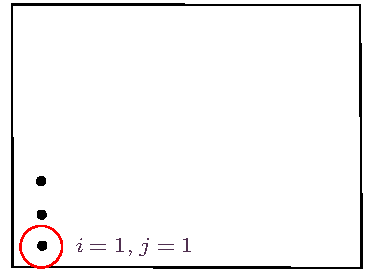
\includegraphics[width=6.54174865538502cm,height=4.62757444575626cm]{slides-8.pdf}}}}
    & {\unrollphantoms{\[ \begin{array}{c}
         u_{\tmmathbf{e}, 1, 1}^n - \frac{t}{x_{\tmmathbf{e}} \lambda_x w_1}
         \left( \tilde{F}_{e_x + \frac{1}{2}, e_y, 1} - f_{\tmmathbf{e},
         \frac{1}{2}, 1} \right) \in \Omega,\\
         u_{\tmmathbf{e}, 1, 1}^n - \frac{t}{y_e \lambda_y w_1} \left(
         \tilde{F}_{e_x, e_y + \frac{1}{2}, 1} - f_{\tmmathbf{e}, 1,
         \frac{1}{2}} \right) \in \Omega .
       \end{array} \]}{\[ \lambda_x = \frac{| s_x^{\tmmathbf{e}} | /
       x_{\tmmathbf{e}}}{| s_x^{\tmmathbf{e}} | / x_{\tmmathbf{e}} + |
       s_y^{\tmmathbf{e}} | / y_{\tmmathbf{e}}}, \qquad \lambda_y = \frac{|
       s_y^{\tmmathbf{e}} | / y_{\tmmathbf{e}}}{| s_x^{\tmmathbf{e}} | /
       x_{\tmmathbf{e}} + | s_y^{\tmmathbf{e}} | / y_{\tmmathbf{e}}} \]}}
    
    \
    
    \ 
  \end{tabularx}}}
\end{frame}}{\begin{frame}
  \frametitle{Low order residual : MUSCL-Hancock}
  
  {\unroll{{\center{\resizebox{0.4\columnwidth}{!}{\includegraphics{slides-9.pdf}}}}}{Integrating
  the conservation law over the subcell $I^e_j$, we get
  \[ x_e w_j  (u_j^{n + 1} - u_j^n) + \int_{t^n}^{t^{n + 1}} (f_{j + 1 / 2} -
     f_{j - 1 / 2}) d \nocomma t = 0. \]}{Using the mid-point rule, writing
  explicit update,
  \[ u_j^{n + 1} = u_j^n - \frac{t}{x_e w_j}  (f_{j + 1 / 2}^{n + 1 / 2} -
     f_{j - 1 / 2}^{n + 1 / 2}) \]}{\[ f_{j + 1 / 2}^{n + 1 / 2} = f (u_{j + 1
     / 2 -}^{n + 1 / 2}, u_{j + 1 / 2 +}^{n + 1 / 2}) \]}{\[ \begin{array}{c}
       u_{j - 1 / 2 +} = u_j (x_{j - 1 / 2}), \quad u_{j + 1 / 2 -} = u_j
       (x_{j + 1 / 2})\\
       u_j (x) = u_j^n + \delta_j \cdot (x - x_j)\\
       \delta_j = \tmop{minmod} \left( \beta_j  \frac{u_{j + 1} - u_j}{x_{j +
       1} - x_j}, D_{\tmop{cent}} (u)_j, \beta_j \frac{u_j^n - u_{j -
       1}^n}{x_j - x_{j - 1}} \right)
     \end{array} \]}{\[ u_{j - \frac{1}{2} +}^{n + 1 / 2} = u_{j - 1 / 2}^n -
     \frac{t}{2} \frac{f (u_{j + 1 / 2}) - f (u_{j - 1 / 2})}{x_{j + 1 / 2} -
     x_{j - 1 / 2}}, \quad u_{j + \frac{1}{2} -}^{n + 1 / 2} = u_{j + 1 / 2}^n
     - \frac{t}{2} \frac{f (u_{j + 1 / 2}) - f (u_{j - 1 / 2})}{x_{j + 1 / 2}
     - x_{j - 1 / 2}} . \]}}
  
  {\tmsamp{}}
\end{frame}}{\begin{frame}
  \frametitle{Admissibility of low order method}
  
  \begin{theorem}
    \tmtextit{$($Extension of Berthon $\cite{Berthon2006} )$} Consider the
    conservation law
    \[ \bw_t + \tmmathbf{f} \left( \bw \right)_x = 0 \]
    which preserves a convex set $\Omega$. Let $\{ \tmmathbf{w}_i^n \}_{i \in
    \mathbb{Z}}$ be the approximate solution at time level $n$ and assume that
    $\tmmathbf{w}^n_i \in \Omega$ for all $i \in \mathbb{Z}$. Consider
    \tmcolor{red}{conservative reconstructions}
    \[ \bw_i^{n, +} = \bw_i + (x_{i + 1 / 2} - x_i) \sigma_i, \quad \bw_i^{n,
       -} = \bw_i + (x_{i - 1 / 2} - x_i) \sigma_i . \]
    Define $\tmmathbf{w}_i^{\ast, \pm}$ satisfying
    \[ \begin{array}{c}
         \tmcolor{red}{\mu^-}  \bw_i^{n, -} + \bw_i^{\ast, \pm} +
         \tmcolor{red}{\mu^+}  \bw_i^{n, +} = 2 \bw_i^{n, \pm},
       \end{array} \]
    where
    \[ \tmcolor{red}{\mu^-} = \frac{x_{i + 1 / 2} - x_i}{x_{i + 1 / 2} - x_{i
       - 1 / 2}}, \quad \tmcolor{red}{\mu^+} = \frac{x_i - x_{i - 1 / 2}}{x_{i
       + 1 / 2} - x_{i - 1 / 2}} . \]
    Assume that the slope $\sigma_i$ is chosen so that
    \[ \bw_i^{\ast, \pm} \in \Omega . \]
    Then, under \tmcolor{blue}{appropriate} time step restrictions, the
    updated solution $\tmmathbf{w}_i^{n + 1}$, defined by the MUSCL-Hancock
    procedure is in $\Omega$.
  \end{theorem}
  
  {\center{\resizebox{0.6\columnwidth}{!}{\includegraphics{slides-10.pdf}}}}
\end{frame}}{\begin{frame}
  \frametitle{Generalizing Berthon's proof}
  
  {\unroll{Berthon defined $\bw_i^{\ast, \pm}$ to be the quantity satisfying
  \[ \frac{1}{2} \bw_i^{n, -} + \bw_i^{\ast, \pm} + \frac{1}{2} \bw_i^{n, +} =
     2 \bw_i^{n, \pm} . \]}{For non-cell centred grids, we generalize to
  \[ \begin{array}{c}
       \tmcolor{red}{\mu^-}  \bw_i^{n, -} + \bw_i^{\ast, \pm} +
       \tmcolor{red}{\mu^+}  \bw_i^{n, +} = 2 \bw_i^{n, \pm},
     \end{array} \]
  where
  \[ \tmcolor{red}{\mu^-} = \frac{x_{i + 1 / 2} - x_i}{x_{i + 1 / 2} - x_{i -
     1 / 2}}, \quad \tmcolor{red}{\mu^+} = \frac{x_i - x_{i - 1 / 2}}{x_{i + 1
     / 2} - x_{i - 1 / 2}} . \]}{This choice was made to get the natural
  expression of $\tmmathbf{w}_i^{\ast, \pm}$ in the \tmtextbf{conservative
  case} -
  \[ \bw_i^{\ast, \pm} = \bw \tmmathbf{w}_i^n + 2 (x_{i \pm 1 / 2} - x_i)
     \sigma_i, \]
  noting that
  \[ \bw_i^{n, +} = \bw_i + (x_{i + 1 / 2} - x_i) \sigma_i, \quad \bw_i^{n, -}
     = \bw_i + (x_{i - 1 / 2} - x_i) \sigma_i . \]}}
  
  \ 
\end{frame}}{\begin{frame}
  \frametitle{Step 1 : Evolution to $n + 1 / 2$}
  
  \begin{lemma}
    \label{lemma:m.h.step.1}\tmtextbf{(Evolution)} Pick
    \[ \tmcolor{red}{\mu^-} = \frac{x_{i + 1 / 2} - x_i}{x_{i + 1 / 2} - x_{i
       - 1 / 2}}, \quad \tmcolor{red}{\mu^+} = \frac{x_i - x_{i - 1 / 2}}{x_{i
       + 1 / 2} - x_{i - 1 / 2}}, \]
    so that
    \[ \frac{\tmcolor{red}{\mu^-}}{2} \bw_i^{n, -} + \frac{1}{2} \bw_i^{\ast,
       \pm} + \frac{\tmcolor{red}{\mu^+}}{2} \bw_i^{n, +} = \bw_i^{n, \pm} .
    \]
    Then, assume that
    \[ \bw_i^{n, \pm} \in \Omega \quad \text{and} \quad \bw_i^{\ast, \pm} \in
       \Omega, \]
    and the CFL restrictions
    \begin{equation}
      \begin{array}{c}
        \frac{t / 2}{\tmcolor{red}{\mu^-} x / 2} \max_{i \in \mathbb{Z}}
        \left( \left| \sigma_e \left( \bw_i^{n, -}, \bw_i^{\ast, \pm} \right)
        \right| \right) \leq \frac{1}{2},\\
        \frac{t / 2}{\tmcolor{red}{\mu^+} x / 2} \max_{i \in \mathbb{Z}}
        \left( \left| \sigma_e \left( \bw_i^{\ast, \pm}, \bw_i^{n, +} \right)
        \right| \right) \leq \frac{1}{2},
      \end{array} \label{eq:new.cfl1}
    \end{equation}
    where $\sigma_e \left( \bw_1, \bw_2 \right)$ denotes all eigenvalues of
    all Jacobian matrices at the states between $\bw_1 \infixand \bw_2$.
    
    Then, we have invariance of $\Omega$ under the first step of MUSCL-Hancock
    scheme, i.e.,
    \[ \bw_i^{n + 1 / 2, \pm} \in \Omega . \]
  \end{lemma}
\end{frame}}{\begin{frame}
  \frametitle{Step 1 : Evolution to $n + 1 / 2$}
  
  {\unroll{{\center{\raisebox{-0.5\height}{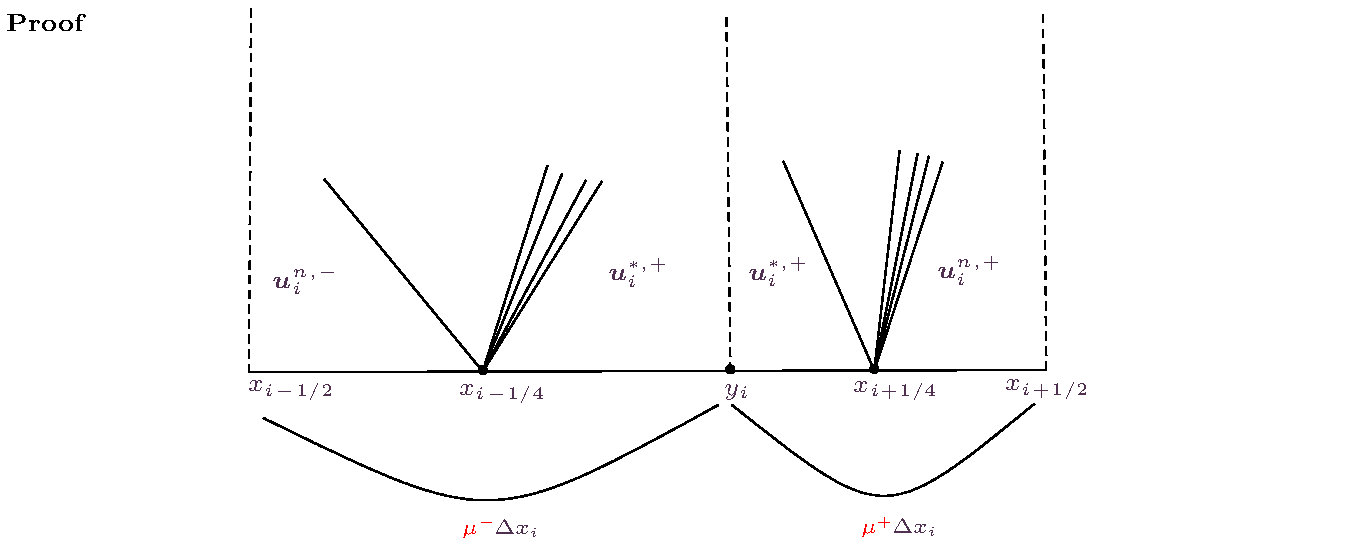
\includegraphics[width=22.9760920897285cm,height=9.25501770956316cm]{slides-11.pdf}}}}}{\[
  \begin{array}{cccc}
       \widetilde{\bw}_i^{n + \frac{1}{2}, +} & = & \frac{1}{x_i} \int_{x_{i -
       1 / 2}}^{x_{i + 1 / 2}} \bw^h (x, t / 2) d x & \\
       & = & \frac{1}{x_i} \left[\begin{array}{c}
         \left( \frac{y_i - x_{i - 1 / 2}}{2} \right) \bw_i^{n, -} +
         \frac{x_i}{2} \bw_i^{\ast, +} + \frac{(x_{i + 1 / 2} - y_i)}{2}
         \bw_i^{n, +} - t / 2 \left( f \left( \bw_i^{n, +} \right) - f \left(
         \bw_i^{n, -} \right) \right)
       \end{array}\right] & \\
       & = & \frac{1}{2} \left( \tmcolor{red}{\mu^-} \tmmathbf{w}_i^{n, -} +
       \bw_i^{\ast, +} + \tmcolor{red}{\mu^+} \bw_i^{n, +} \right) - \frac{t /
       2}{x_i} \left( f \left( \bw_i^{n, +} \right) - f \left( \bw_i^{n, -}
       \right) \right) & \\
       & = & \bw_i^{n, +} - \frac{t / 2}{x_i} \left( f \left( \bw_i^{n, +}
       \right) - f \left( \bw_i^{n, -} \right) \right) = \bw_i^{n +
       \frac{1}{2}, +} & \qed
     \end{array} \]}}
  
  \ 
\end{frame}}{\begin{frame}
  \frametitle{Step 2 : FVM type update}
  
  {\unroll{{\small{We introduce a new variable $\tmmathbf{w}_i^{n +
  \frac{1}{2}, \ast}$ defined so that}}
  \[ \small{\tmcolor{red}{\mu^-} \bw_i^{n + \frac{1}{2}, -} + \bw_i^{n +
     \frac{1}{2}, \ast} + \tmcolor{red}{\mu^+} \bw_i^{n + \frac{1}{2}, \ast} =
     2 \bw_i^n .}
  \]}{\raisebox{-0.5\height}{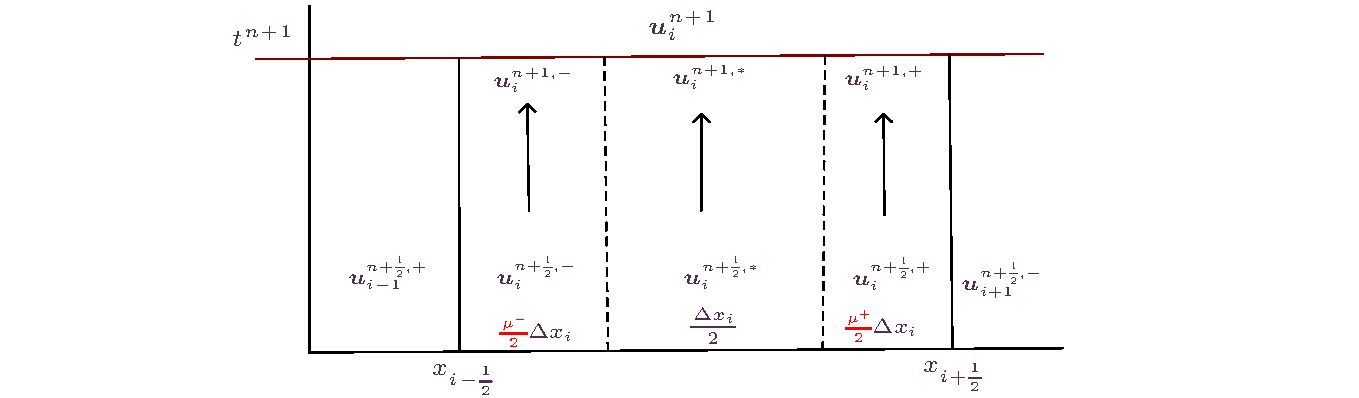
\includegraphics[width=22.8239210284665cm,height=6.67689885871704cm]{slides-12.pdf}}}{{\small{\[
  \begin{array}{ccc}
       \bw_i^{n + 1, -} & : = & \bw_i^{n + \frac{1}{2}, -} -
       \cfrac{t}{\tmcolor{red}{\mu^-} x_i / 2} \left( f \left( \bw_i^{n +
       \frac{1}{2}, -}, \bw_i^{n + \frac{1}{2}, \ast} \right) - f \left(
       \bw_{i - 1}^{n + \frac{1}{2}, +}, \bw_i^{n + \frac{1}{2}, -} \right)
       \right)\\
       \bw_i^{n + 1, \ast} & : = & \bw_i^{n + \frac{1}{2}, \ast} -
       \cfrac{t}{x_i / 2} \left( f \left( \bw_i^{n + \frac{1}{2}, \ast},
       \bw_i^{n + \frac{1}{2}, +} \right) - f \left( \bw_i^{n + \frac{1}{2},
       -}, \bw_i^{n + \frac{1}{2}, \ast} \right) \right)\\
       \bw_i^{n + 1, +} & : = & \bw_i^{n + \frac{1}{2}, +} -
       \cfrac{t}{\tmcolor{red}{\mu^+} x_i / 2} \left( f \left( \bw_i^{n +
       \frac{1}{2}, +}, \bw_{i + 1}^{n + \frac{1}{2}, -} \right) - f \left(
       \bw_i^{n + \frac{1}{2}, \ast}, \bw_i^{n + \frac{1}{2}, +} \right)
       \right)
     \end{array} \]}}}{\[ \small{\bw_i^{n + 1} = \bw_i^n - \frac{t}{x} \left(
     \tmmathbf{f} \left( \bw_i^{n + \frac{1}{2}, +}, \bw_{i + 1}^{n +
     \frac{1}{2}, -} \right) - \tmmathbf{f} \left( \bw_{i - 1}^{n +
     \frac{1}{2}, +}, \bw_i^{n + \frac{1}{2}, -} \right) \right)} \]}}
  
  \ 
\end{frame}}{\begin{frame}
  \frametitle{Step 2 : FVM type update}
  
  {\unroll{\begin{lemma}
    \label{lemma:muscl.step2.general}$($\tmtextbf{Riemann solver}$)$ Assume
    that the states $\left( \bw_i^{n + \frac{1}{2}, \pm} \right)_{i \in
    \mathbb{Z}}$, $\left( \bw_i^{n + \frac{1}{2}, \ast} \right)_{i \in
    \mathbb{Z}}$ belong to $\Omega$, where $\bw_i^{n + \frac{1}{2}, \ast}$ was
    defined above as
    \[ \tmcolor{red}{\mu^-} \bw_i^{n + \frac{1}{2}, -} + \bw_i^{n +
       \frac{1}{2}, \ast} + \tmcolor{red}{\mu^+} \bw_i^{n + \frac{1}{2}, +} =
       2 \bw_i^n . \]
    Then, the updated solution of MUSCL-Hancock scheme is in $\Omega$ under
    the CFL conditions
    \begin{equation}
      \begin{array}{c}
        \cfrac{t}{\tmcolor{red}{\mu^-} x_i / 2} \max_{i \in \mathbb{Z}} 
        \left( \left| \sigma_e \left( \bw_i^{n + \frac{1}{2}, -}, \bw_i^{n +
        \frac{1}{2}, \ast} \right) \right| \right) \leq \frac{1}{2},\\
        \cfrac{t}{\tmcolor{red}{\mu^-} x_i / 2} \max_{i \in \mathbb{Z}} 
        \left( \left| \sigma_e \left( \bw_{i - 1}^{n + \frac{1}{2}, +},
        \bw_i^{n + \frac{1}{2}, -} \right) \right| \right) \leq \frac{1}{2},\\
        \\
        \cfrac{t}{x_i / 2} \max_{i \in \mathbb{Z}}  \left( \left| \sigma_e
        \left( \bw_i^{n + \frac{1}{2}, \ast}, \bw_i^{n + \frac{1}{2}, +}
        \right) \right| \right) \leq \frac{1}{2},\\
        \cfrac{t}{x_i / 2} \max_{i \in \mathbb{Z}}  \left( \left| \sigma_e
        \left( \bw_i^{n + \frac{1}{2}, -}, \bw_i^{n + \frac{1}{2}, \ast}
        \right) \right| \right) \leq \frac{1}{2},\\
        \\
        \cfrac{t}{\tmcolor{red}{\mu^+} x_i / 2} \max_{i \in \mathbb{Z}} 
        \left( \left| \sigma_e \left( \bw_i^{n + \frac{1}{2}, +}, \bw_{i +
        1}^{n + \frac{1}{2}, -} \right) \right| \right) \leq \frac{1}{2},\\
        \cfrac{t}{\tmcolor{red}{\mu^+} x_i / 2} \max_{i \in \mathbb{Z}} 
        \left( \left| \sigma_e \left( \bw_i^{n + \frac{1}{2}, \ast}, \bw_i^{n
        + \frac{1}{2}, +} \right) \right| \right) \leq \frac{1}{2} .
      \end{array} \label{eq:new.cfl2}
    \end{equation}
  \end{lemma}}}
  
  {\unroll{\ }}
  
  \ 
\end{frame}}{\begin{frame}
  \frametitle{Final admissibility condition}
  
  {\unroll{{\switch{}{}{\[ \bw_i^{n + \frac{1}{2}, \ast} = \left(
     \underbrace{2 \bw_i^n - \left( \tmcolor{red}{\mu^-} \bw_i^{n, -} +
     \tmcolor{red}{\mu^+} \bw_i^{n, +} \right)}_{\bw_i^n} \right) - \frac{t}{2
     x} \left[ \left( f \left( \tmcolor{blue}{\tmmathbf{\bw}_i^{n, -}} \right)
     - f \left( \tmcolor{blue}{\tmmathbf{\bw}_i^{n, +}} \right) \right)
     \right] \]}}}{\begin{lemma}
    \label{lemma:muscl.step3.wss}$($\tmtextbf{Link previous lemmas}$)$ Assume
    that $\bw_i^n \in \Omega$ for all $i \in \mathbb{Z}$. Let us define
    $\bw_i^{\ast, \ast}$ as follows:
    \begin{equation}
      \tmcolor{red}{\mu^-} \bw_i^{n, -} + \bw_i^{\ast, \ast} +
      \tmcolor{red}{\mu^+} \bw_i^{n, +} = 2 \left( 2 \bw_i^n - \left(
      \tmcolor{red}{\mu^-} \bw_i^{n, -} + \tmcolor{red}{\mu^+} \bw_i^{n, +}
      \right) \right), \label{eq:lemma.1.used}
    \end{equation}
    where, as defined before,
    \[ \tmcolor{red}{\mu^-} = \frac{x_{i + 1 / 2} - x_i}{x_{i + 1 / 2} - x_{i
       - 1 / 2}}, \quad \tmcolor{red}{\mu^+} = \frac{x_i - x_{i - 1 / 2}}{x_{i
       + 1 / 2} - x_{i - 1 / 2}} . \]
    Assume that $\bw_i^{n, \pm}$ and $\bw_i^{\ast, \ast}$ are in $\Omega$.
    Consider the CFL conditions
    \begin{equation}
      \begin{array}{l}
        \frac{t / 2}{\tmcolor{red}{\mu^-} x / 2} \max_{i \in \mathbb{Z}}
        \left( \left| \sigma_e \left( \bw_i^{\ast, \ast}, \bw_i^{n, -} \right)
        \right| \right) \leq \frac{1}{2},\\
        \frac{t / 2}{\tmcolor{red}{\mu^+} x / 2} \max_{i \in \mathbb{Z}}
        \left( \left| \sigma_e \left( \bw_i^{n, +}, \bw_i^{\ast, \ast} \right)
        \right| \right) \leq \frac{1}{2},
      \end{array} \label{eq:new.cfl3}
    \end{equation}
    then $\bw_i^{n + \frac{1}{2}, \ast} \in \Omega$.
  \end{lemma}}{\begin{remark}
    For conservative reconstruction, we actually have $\tmmathbf{\bw}_i^{\ast,
    \ast} = \bw_i$.
  \end{remark}}}
  
  \ 
\end{frame}}{\begin{frame}
  \frametitle{Final admissibility condition}
  
  {\unroll{\raisebox{-0.5\height}{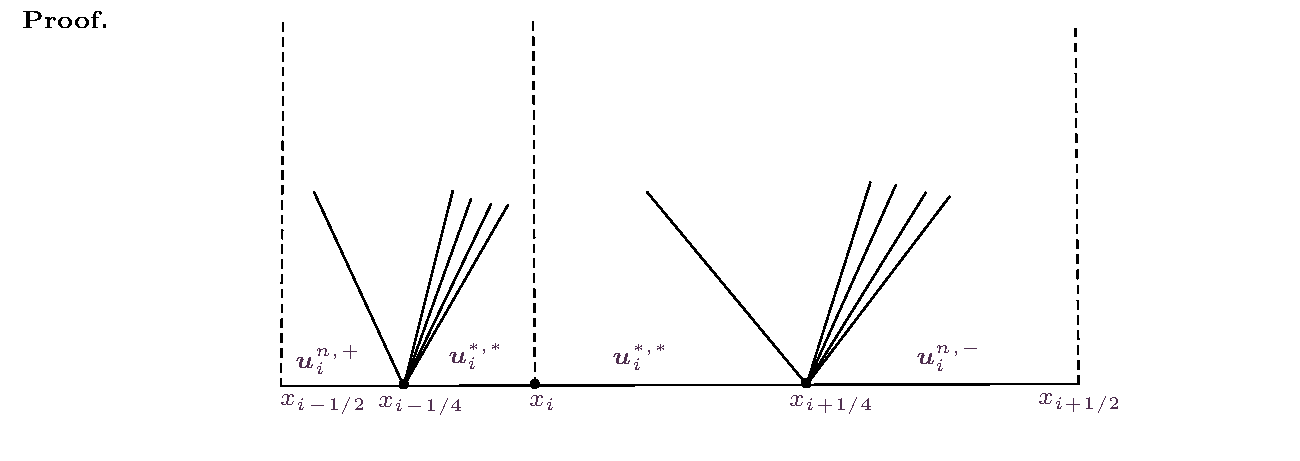
\includegraphics[width=21.8323494687131cm,height=7.73448773448773cm]{slides-13.pdf}}}{\[
  \begin{array}{ccc}
       \widetilde{\bw}_i^{n + \frac{1}{2}, \ast} & = & \frac{1}{x_i}
       \int_{x_{i - 1 / 2}}^{x_{i + 1 / 2}} \bw^h \left( x, \frac{t}{2}
       \right) d \nocomma x\\
       & = & \frac{1}{x_i} \left(\begin{array}{c}
         \left( \frac{x_i - x_{i - 1 / 2}}{2} \right) \bw_i^{n, +} +
         \frac{x_i}{2} \bw_i^{\ast, \ast} + \frac{(x_{i + 1 / 2} - x_i)}{2}
         \bw_i^{n, -}\\
         \quad - \frac{t}{2} \left( f \left( \bw_i^{n, -} \right) - f \left(
         \bw_i^{n, +} \right) \right)
       \end{array}\right)\\
       & = & \frac{1}{2} \left( \tmcolor{red}{\mu^+} \tmmathbf{w}_i^{n, +} +
       \bw_i^{\ast, \ast} + \tmcolor{red}{\mu^-} \bw_i^{n, -} \right) -
       \frac{t / 2}{x_i} \left( f \left( \bw_i^{n, -} \right) - f \left(
       \bw_i^{n, +} \right) \right)\\
       & = & \bw_i^{n + \frac{1}{2}, \ast}
     \end{array} \]}}
\end{frame}}{\frametitle{Final admissibility condition}

{\unroll{\begin{theorem}
  Consider the conservation law
  \[ \bw_t + \tmmathbf{f} \left( \bw \right)_x = 0 \]
  which  preserves a convex set $\Omega$. Let $\left\{ \bw_i^n \right\}_{i \in
  \mathbb{Z}}$ be the approximate solution at time level $n$ and assume that
  $\bw^n_i \in \Omega$ for all $i \in \mathbb{Z}$. Consider
  \tmcolor{red}{conservative reconstructions}
  \[ \bw_i^{n, +} = \bw_i + (x_{i + 1 / 2} - x_i) \sigma_i, \quad \bw_i^{n, -}
     = \bw_i + (x_{i - 1 / 2} - x_i) \sigma_i . \]
  Define $\tmmathbf{w}_i^{\ast, \pm}$ to be
  \[ \bw_i^{\ast, \pm} = \bw_i^n + 2 \left( x_{i \pm \frac{1}{2}} - x_i
     \right) \sigma_i \]
  and assume that the slope $\sigma_i$ is chosen so that
  \[ \bw_i^{\ast, \pm} \in \Omega . \]
  Then, under time step restrictions {\eqref{eq:new.cfl1}},
  {\eqref{eq:new.cfl2}}, {\eqref{eq:new.cfl3}}, the updated solution $\bw_i^{n
  + 1}$, defined by the MUSCL-Hancock procedure is in $\Omega$.
\end{theorem}}{{\hidden*{\begin{proof}
  We only need $\bw_i^{n, \pm} \in \Omega$ to apply the previous lemmas. To
  that end, notice
  \[ \bw_i^{n, \pm} = \frac{1}{2} \bw_i^{\ast, \pm} + \frac{1}{2} \bw_i^n . \]
\end{proof}}}}}

\

\ }{\begin{frame}
  \frametitle{Enforcing slope restriction}
  
  {\unroll{We are given that $\bw_i^n \in \Omega$ and a candidate slope
  $\tmmathbf{\sigma}_i$. We have to limit it so that
  \[ \bw_i^{\ast, \pm} = \bw_i^n + 2 (x_{i \pm 1 / 2} - x_i)
     \tmmathbf{\sigma}_i \in \Omega . \]}{We shall do this by finding a
  $\theta \in [0, 1]$ such that
  \begin{equation}
    \bw_i^n +^{} \theta (2 (x_{i \pm 1 / 2} - x_i) \tmmathbf{\sigma}_i) \in
    \Omega . \label{eq:admissible.theta.defn}
  \end{equation}}{We assume that there is a a concave function $p = p \left(
  \bw \right)$ such that the admissibility criterion is given by
  \[ p \left( \bw \right) > 0. \]}{We pick
  \[ \theta_{\pm} = \min \left( \left| \frac{\epsilon - p \left( \bw_i^n
     \right)}{p \left( \bw_i^{\ast, \pm} \right) - p \left( \bw_i^n \right)}
     \right|, 1 \right) \]
  and
  \[ \theta = \min (\theta_+, \theta_-) . \]
  By Jensen's inequality, this $\theta$ will give us
  {\eqref{eq:admissible.theta.defn}}. This approach is used when using
  Zhang-Shu's positivty limiter {\cite{Zhang2010b}} in practice.}}
\end{frame}}{\begin{frame}
  \frametitle{Non-conservative reconstruction}
  
  Consider non-conservative variables
  \[ \tmmathbf{U}_i^n = \kappa \left( \bw_i^n \right), \]
  so that reconstruction is given by
  \[ \tmmathbf{U}^n (x) = \tmmathbf{U}^n_i + \sigma_i (x - x_i) \]
  \begin{equation}
    \begin{array}{ccc}
      \bw_i^{n, \pm} & : = & \kappa^{- 1} (\tmmathbf{U}_i^{n, \pm})
    \end{array} \label{eq:non.con.face.defn1}
  \end{equation}
  \begin{theorem}
    Assume that $\bw_i^n \in \Omega$ for all $i \in \mathbb{Z}$. Consider
    $\bw_i^{n, \pm}$ defined in $\eqref{\tmop{eq} : \tmop{non} . \tmop{con} .
    \tmop{face} . \tmop{defn} 1}$, $\bw_i^{\ast, \pm}$ defined so that
    \[ \mu^- \bw_i^{n + \frac{1}{2}, -} + \bw_i^{n + \frac{1}{2}, \ast} +
       \mu^+ \bw_i^{n + \frac{1}{2}, +} = 2 \bw_i^n, \]
    and $\bw_i^{\ast, \ast}$ defined explicitly as
    \[ \bw_i^{\ast, \ast} = 4 \bw_i^n - 3 \left( \mu^- \bw_i^{n, -} + \mu^+
       \bw_i^{n, +} \right) . \]
    Assume that the slope is chosen so that
    \[ \bw_i^{n, \pm} \in \Omega, \quad \bw_i^{\ast, \pm} \in \Omega \quad
       \tmop{and} \quad \tmmathbf{\bw}_i^{\ast, \ast} \in \Omega . \]
    Consider the same CFL conditions {\eqref{eq:new.cfl1}},
    {\eqref{eq:new.cfl2}}, {\eqref{eq:new.cfl3}}. Then the updated solution
    $\bw_i^{n + 1}$ of MUSCL-Hancock procedure is in $\Omega$.
  \end{theorem}
  
  \begin{remark}
    The definition of $\tmmathbf{w}_i^{\ast, \ast}$ comes from
    \[ \tmcolor{red}{\mu^-} \bw_i^{n, -} + \bw_i^{\ast, \ast} +
       \tmcolor{red}{\mu^+} \bw_i^{n, +} = 2 \left( 2 \bw_i^n - \left( \mu^-
       \bw_i^{n, -} + \mu^+ \bw_i^{n, +} \right) \right) \]
  \end{remark}
\end{frame}}{\begin{frame}
  \frametitle{ADER-DG : Predictor step}
  
  {\unroll{Current solution
  \[ x \in I_e : \qquad u_h^n (\xi) = \sum_{j = 1}^{N + 1} u_j^n \ell_j (\xi)
  \]}{Cell local space-time solution and flux: $\tau = (t - t_n) / t$
  \[ \tilde{u}_h (\xi, \tau) = \sum_{r, s = 1}^{N + 1} \tilde{u}_{r s} \ell_r
     (\xi) \ell_s (\tau), \quad \tilde{f}_h (\xi, \tau) = \sum_{r, s = 1}^{N +
     1} f (\tilde{u}_{r \nocomma s}) \ell_r (\xi) \ell_s (\tau) . \]}{Find
  $\tilde{u}_h$ by cell local Galerkin method
  \[ \int_{t_n}^{t_{n + 1}} \int_{I_e} (\partial_t \tilde{u}_h + \partial_x
     \tilde{f}_h) \ell_r (\xi) \ell_s (\tau) d \nocomma x d \nocomma t, \qquad
     1 \leq r, s \leq N + 1. \]}{Integrate by parts in time
  \[ \begin{array}{c}
       - \int_{t_n}^{t_{n + 1}} \int_{I_e} \tmcolor{red}{\tilde{u}_h} \ell_r
       (\xi) \partial_t \ell_s (\tau) d x d t + \int_{I_e}
       \tmcolor{red}{\tmcolor{red}{\tilde{u}_h} (\xi, 1)} \ell_r (\xi) \ell_s
       (1) d x - \int_{I_e} \tmcolor{blue}{u_h^n (\xi)} \ell_r (\xi) \ell_s
       (0) d \xi\\
       + \int_{t_n}^{t_{n + 1}} \int_{I_e} \partial_x \tilde{f}_h \ell_r (\xi)
       \ell_s (\tau) d x d t = 0.
     \end{array} \]}}
\end{frame}}{\begin{frame}
  \frametitle{ADER correction step}
  
  {\unroll{\[ \int_{t_n}^{t_{n + 1}} \int_0^1 (\partial_t u_h + \partial_x f
     (u_h)) \ell_i (\xi) d x d t = 0 \]}{Integrate by parts :
  \[ \begin{array}{ccc}
       \int_{I_e} u_h^{n + 1} \ell_i (\xi) d x & = & \int_{I_e} u_h^n \ell_i
       (\xi) d x + \int_{t^n}^{t^{n + 1}} \int_{I_e} \tilde{f}_h \partial_x
       \ell_i (\xi) d x d t\\
       &  & \quad + \int_{t^n}^{t^{n + 1}} f (\tilde{u}_{e - \frac{1}{2}}^-
       (t), \tilde{u}_{e - \frac{1}{2}}^+ (t)) \ell_i (0) d t -
       \int_{t^n}^{t^{n + 1}} f (\tilde{u}_{e + \frac{1}{2}}^- (t),
       \tilde{u}_{e + \frac{1}{2}}^+ (t)) \ell_i (1) d t.
     \end{array} \]}{Another integration by parts :
  \[ \begin{array}{lll}
       \int_{I_e} u_h^{n + 1} \ell_i (\xi) d x & = & \int_{I_e} u_h^n \ell_i
       (\xi) d x - \int_{t^n}^{t^{n + 1}} \int_{I_e} \partial_x \tilde{f}_h
       \ell_i (\xi) d x d t\\
       &  & + \int_{t^n}^{t^{n + 1}} \left( f (\tilde{u}_{e - \frac{1}{2}}^-
       (t), \tilde{u}_{e - \frac{1}{2}}^+ (t)) - \tilde{f}_h (0, \tau) \right)
       \ell_i (0) d t\\
       &  & - \int_{t^n}^{t^{n + 1}} \left( f (\tilde{u}_{e + \frac{1}{2}}^-
       (t), \tilde{u}_{e + \frac{1}{2}}^+ (t)) - \tilde{f}_h (1, \tau) \right)
       \ell_i (1) d t,
     \end{array} \]}{Quadrature on solution points :
  
  {\switch{}{\[ \begin{array}{cccc}
       &  &  & u_i^n - \int_{t^n}^{t^{n + 1}} \partial_x \tilde{f}_h (\xi_i,
       \tau) d t\\
       \Rightarrow & u_i^{n + 1} & = & \quad - \tmcolor{red}{g_L' (\xi_i)}
       \int_{t^n}^{t^{n + 1}} f (\tilde{u}_{e - \frac{1}{2}}^- (t),
       \tilde{u}_{e - \frac{1}{2}}^+ (t)) - \tilde{f}_h (0, \tau) d t\\
       &  &  & \quad - \tmcolor{red}{g_R' (\xi_i)} \int_{t^n}^{t^{n + 1}} f
       (\tilde{u}_{e + \frac{1}{2}}^- (t), \tilde{u}_{e + \frac{1}{2}}^+ (t))
       - \tilde{f}_h (1, \tau) d t
     \end{array} \]}}}}
\end{frame}}{\begin{frame}
  \frametitle{ADER and LWFR for constant linear advection}
  
  {\unroll{For constant linear advection
  \[ u_t + u_x = 0, \]
  the ADER update is given by
  \begin{equation}
    \begin{array}{ccc}
      &  & u_i^n - \partial_x \int_{t^n}^{t^{n + 1}} \tilde{u}_h (\xi_i,
      \tau) d t\\
      u_i^{n + 1} & = & \quad - g_L' (\xi_i) \left[ f \left( \int_{t^n}^{t^{n
      + 1}} \tilde{u}_{e - \frac{1}{2}}^- (t) d t, \int_{t^n}^{t^{n + 1}}
      \tilde{u}_{e - \frac{1}{2}}^+ (t) d t \right) - \int_{t^n}^{t^{n + 1}}
      \tilde{u}_h (0, \tau) d t \right]\\
      &  & \quad - g_R' (\xi_i) \left[ f \left( \int_{t^n}^{t^{n + 1}}
      \tilde{u}_{e + \frac{1}{2}}^- (t) d t, \int_{t^n}^{t^{n + 1}}
      \tilde{u}_{e + \frac{1}{2}}^+ (t) d t \right) - \int_{t^n}^{t^{n + 1}}
      \tilde{u}_h (1, \tau) d t \right]
    \end{array} \label{eq:ader.linear.update}
  \end{equation}}{The LWFR update is given by
  \begin{equation}
    u_i^{n + 1} = u_i^n - \partial_x U_h (\xi_i) - g_L' (\xi_i) \left[ f (U_{e
    - \frac{1}{2}}^-, U_{e - \frac{1}{2}}^+) - U_h (0) \right] - g_R' (\xi_i)
    \left[ f (U_{e + \frac{1}{2}}^-, U_{e + \frac{1}{2}}^+) - U_h (1) \right],
    \label{eq:lwfr.linear.update}
  \end{equation}
  where
  \[ \begin{array}{ccc}
       U_h^n & = & u + \frac{t}{2} u_t + \frac{t^2}{3!} u_{t \nocomma t} +
       \cdots + \frac{t^N}{(N + 1) !} \pdv*{N}{u}{t}\\
       & = & u - \frac{t}{2} u_x + \frac{t^2}{3!} u_{x \nocomma x} + \cdots +
       (- 1)^N \frac{t^N}{(N + 1) !} \pdv*{N}{u}{x} .
     \end{array} \]}}
\end{frame}}{\begin{frame}
  \frametitle{Equivalence of ADER-FR and LWFR for linear case}
  
  {\unroll{\begin{theorem}
    For the linear advection equation
    \[ u_t + u_x = 0, \]
    the Lax-Wendroff Flux Reconstruction scheme with D2 dissipation and
    ADER-FR scheme are equivalent.
  \end{theorem}}{\tmtextbf{Proof.} Let $u_e^n = u_e^n (x)$ denote the solution
  polynomial at time level $n$ in element $e$.}{Then, \ $\tilde{u}_h (x, t) :
  = u_e^n (x - (t - t^n))$ is a weak solution of the equation
  \[ \begin{array}{cccc}
       \tilde{u}_t + \tilde{u}_x & = & 0, & x \in [x_{e - 1 / 2}, x_{e + 1 /
       2}], t \in (t_n, t_{n + 1}],\\
       \tilde{u} (x, t^n) & = & u^n_e (x), & t = t_n .
     \end{array} \]}{Since the predictor equation has a \tmcolor{red}{unique}
  solution of degree $N$ {\cite{Jackson2017,Dumbser2009}}, the specified
  $\tilde{u}_h$ must be \tmcolor{red}{the} predictor solution.}{{\unroll{\[ 
     \begin{array}{cccc}
       & \tilde{u}_h (x, t) & = & \tilde{u}_h (x, t^n) + (t - t^n) \pdv{}{t}
       \tilde{u}_h (x, t^n) + \ldots + \frac{(t - t^n)^N}{N!} \pdv*{N}{}{t}
       \tilde{u}_h (x, t^n)\\
       &  & = & u^n (x) - (t - t^n)  \pdv{}{x} u^n (x) + \ldots + (- 1)^N
       \frac{(t - t^n)^N}{N!} \pdv*{N}{}{x} u^n (x)\\
       \Rightarrow &  \frac{1}{t} \int_{t^n}^{t^{n + 1}} \tilde{u}_h (x, t) d
       t & = & u^n (x) - \frac{t}{2}  \pdv{}{x} u_{}^n (x) + \ldots + (- 1)^N
       \frac{t^N}{(N + 1) !} \pdv*{N}{}{x} u^n d t,\\
       \Rightarrow &  \frac{1}{t} \int_{t^n}^{t^{n + 1}} \tilde{u}_h (x, t) d
       t & = & U_h^n (x)
     \end{array} \]
  
  Thus, the ADER-update {\eqref{eq:ader.linear.update}} and the LWFR-update
  {\eqref{eq:lwfr.linear.update}} are the same.\qquad{\qed}}}}}
  
  \
  
  \ 
\end{frame}}{\begin{frame}
  \frametitle{Numerical verification of equivalence of ADER and LW-D2}
  
  \begin{figure}[h]
    {\noindent}\begin{tabularx}{1.0\textwidth}{@{}X@{}@{}X@{}}
      \resizebox{0.35\columnwidth}{!}{\includegraphics{slides-14.pdf}} &
      \resizebox{0.35\columnwidth}{!}{\includegraphics{slides-15.pdf}}\\
      $N = 1$ & $N = 2$\\
      \resizebox{0.35\columnwidth}{!}{\includegraphics{slides-16.pdf}} &
      \resizebox{0.35\columnwidth}{!}{\includegraphics{slides-17.pdf}}\\
      $N = 3$ & $N = 4$
    \end{tabularx}
    \caption{$L^2$ error comparison of ADER, LWFR and RKFR for linear
    advection equation with \tmtextbf{wave packet} initial data $u_0 (x) =
    e^{- 10 x^2} \sin (10 \pi x)$ and \tmtextbf{periodic boundary conditions}
    on $[- 1, 1]$ with $120$ degrees of freedom each.}
  \end{figure}
\end{frame}}{\begin{frame}
  \frametitle{Numerical verification of equivalence of ADER and LW-D2}
  \[ \| u (t) \|^{\ast}_2 \assign \frac{\| u (t) \|_2 - \| u (0) \|_2}{\| u
     (0) \|_2} \]
  \begin{figure}[h]
    {\noindent}\begin{tabularx}{1.0\textwidth}{@{}X@{}@{}X@{}}
      \resizebox{0.32\columnwidth}{!}{\includegraphics{slides-18.pdf}} &
      \resizebox{0.32\columnwidth}{!}{\includegraphics{slides-19.pdf}}\\
      $N = 1$ & $N = 2$\\
      \resizebox{0.32\columnwidth}{!}{\includegraphics{slides-20.pdf}} &
      \resizebox{0.32\columnwidth}{!}{\includegraphics{slides-21.pdf}}\\
      $N = 3$ & $N = 4$ in semi-log scales
    \end{tabularx}
    \caption{Energy comparison of ADER, LWFR and RKFR for linear advection
    equation with \tmtextbf{smooth initial data} $u_0 (x) = \sin (2 \pi x)$
    and \tmtextbf{periodic boundary conditions} on $[- 1, 1]$ with $120$
    degrees of freedom each.}
  \end{figure}
\end{frame}}{\begin{frame}
  \frametitle{ADER-FR and LWFR for non-linear case}
  
  {\unroll{\begin{theorem}
    If the predictor solution of ADER satisfies
    \[ \| U^n \|_{C^{N + 1}} \leq C \]
    where $C$ is a constant independent of $n, x, t$, then the ADER and LW
    solution will satisfy
    \[ \| u^{n + 1}_{\tmop{ADER}} - u^{n + 1}_{\tmop{LW}} \|_{\infty} = O
       (x^{N + 1}) . \]
  \end{theorem}}{{\hidden*{\tmtextbf{Idea of proof.} The weak formulation will
  give us
  \begin{equation}
    \tilde{u}_t + (\tilde{f}_h)_x = 0, \label{eq:quadrature1}
  \end{equation}
  for all $(x_r, t_s)$ where $s > 0$, i.e., $t_s > t^n$. Then, we can
  extrapolate to $t = t^n$ as}}}{{\hidden*{\[ \tilde{u}_t + (\tilde{f}_h)_x =
     O (t^N) \qquad \text{at}  \quad t = t^n, \]}}}{{\hidden*{so that we will
  have
  \[ \begin{array}{rll}
       \tilde{u}_h (x, t^n) & = & \tilde{u}_h (x, t^n) + t (\tilde{f}_h)_x +
       \ldots + \frac{t^N}{N!}  \pdv*{N - 1}{}{t} (\tilde{f}_h)_x + O (t^{N +
       1}) .
     \end{array} \]}}}}
  
  \ 
\end{frame}}{\begin{frame}
  \
  
  \
  
  \
  
  \
  
  \
  
  \
  
  \
  
  \begin{center}
    \ 
  \end{center}
  
  \
  
  \title{Numerical Results}
  
  \maketitle
  
  \ 
\end{frame}}{\begin{frame}
  \
  
  \
  
  \
  
  \
  
  \
  
  \
  
  \
  
  \begin{center}
    \ 
  \end{center}
  
  \
  
  \title{$u_t + u_x = 0$}
  
  \maketitle
  
  \ 
\end{frame}}{\begin{frame}
  \frametitle{Convergence of pure MUSCL-Hancock method}
  \[ \begin{array}{ccccc}
       u_t + u_x & = & 0, & \quad & x \in [- 1, 1], \quad t > 0,\\
       u_0 (x) & = & \sin (2 \pi x), &  & x \in [- 1, 1] .
     \end{array} \]
  {\center{\begin{figure}[h]
    \resizebox{0.5\columnwidth}{!}{\includegraphics{slides-22.pdf}}
    \caption{Convergence test of MUSCL-Hancock setting all $\alpha_e = 1$
    showing close to second order convergence}
  \end{figure}}}
\end{frame}}{\begin{frame}
  \frametitle{Optimal convergence with limiter}
  \[ \begin{array}{ccccc}
       u_t + u_x & = & 0, & \quad & x \in [- 2, 2], \quad t > 0,\\
       u_0 (x) & = & e^{- 10 x^2} \sin (10 \pi x), &  & x \in [- 2, 2] .
     \end{array} \]
  \begin{figure}[h]
    \resizebox{0.5\columnwidth}{!}{\includegraphics{slides-23.pdf}}
    \caption{Convergence analysis with wave packet test case for $N = 3, 4$ at
    $t = 1$}
  \end{figure}
\end{frame}}{\begin{frame}
  \frametitle{Handling discontinuities}
  
  {\center{\tmfloat{h}{small}{figure}{\resizebox{0.6511\columnwidth}{!}{\includegraphics{slides-24.pdf}}}{Composite
  signal {\cite{Jiang1996}} on a mesh of 60 cells for $N = 4$ comparing TVB
  limiter with parameter $M = 50$ and MUSCL-Hancock (MH) blending. Here, the
  smoothness indicator function has been set with $\beta_1 = 0.1$ and $\beta_2
  = 1.0$.}}}
  \[ \begin{array}{ccccc}
       u_t + u_x & = & 0, & \quad & x \in [- 1, 1], \quad t > 0,\\
       u (x, 0) & = & u_0 (x), &  & x \in [- 1, 1],
     \end{array} \]
  \[ \begin{array}{cc}
       \begin{array}{rccc}
         u_0 (x) & = & \left\{\begin{array}{lll}
           G (x, \beta, z), & \qquad & x \in [- 0.8, 0.6],\\
           1, &  & x \in [- 0.4, - 0.2],\\
           1 - | 10 (x - 0.1) |, &  & x \in [0, 0.2],\\
           F (x, \alpha, a), &  & x \in [0.4, 0.6],\\
           0, &  & \tmop{elsewhere},
         \end{array}\right. & x \in [- 1, 1],
       \end{array} & \begin{array}{c}
         G (x, \beta, z) = e^{- \beta (x - z)^2}, \quad F (x, \alpha, a) =
         \sqrt{1 - \alpha^2 (x - a)^2}\\
         a = 0.5, \quad z = - 0.7, \quad \delta = 0.005, \quad \alpha = 10,
         \quad \beta = \frac{\log 2}{36 \delta^2} .
       \end{array}
     \end{array} \]
\end{frame}}{\begin{frame}
  {\switch{\
  
  \
  
  \
  
  \
  
  \title{{\huge{1-D Euler's equations}}}
  
  \maketitle
  
  \
  
  \
  
  
  \[ \frac{\partial}{\partial t} \left(\begin{array}{c}
       \rho\\
       \rho v\\
       E
     \end{array}\right) + \frac{\partial}{\partial x} \left(\begin{array}{c}
       \rho v\\
       p + \rho v^2\\
       (E + p) v
     \end{array}\right) =\tmmathbf{0} \]
  where $\rho, v, p$ and $E$ denote the density, velocity, pressure and total
  energy of the gas, respectively. For a polytropic gas, an equation of sate
  $E = E (\rho, v, p)$ which forms the system closed is given as
  \[ E = E (\rho, v, p) = \frac{p}{\gamma - 1} + \frac{1}{2} \rho v^2 . \]}}
\end{frame}}{\begin{frame}
  \frametitle{Shu-Osher}
  
  \begin{figure}[h]
    \resizebox{0.6\columnwidth}{!}{\includegraphics{slides-25.pdf}}
    \caption{Density profile of Shu-Osher test case {\cite{Shu1989}} at $t =
    1.8$ for accuracy comparison of TVB limiter $\left( M = 300,
    \cite{Qiu2005b} \right)$, blending limiter with MUSCL-Hancock (MH) and
    First Order (FO) blending for degree $N = 4$ on a grid of $400$ cells.}
  \end{figure}
  
  Transmissive boundary conditions on $[- 5, 5]$ with
  \[ (\rho, v, p) = \left\{\begin{array}{lll}
       (3.857143, 2.629369, 10.333333), & \quad & \tmop{if} x < - 4,\\
       (1 + 0.2 \sin (5 x), 0, 1), &  & \tmop{if} x \geq - 4,
     \end{array}\right. \]
  and solution is plotted at $t = 1.8$.
\end{frame}}{\begin{frame}
  \frametitle{Blast}
  
  \begin{figure}[h]
    \resizebox{0.6\columnwidth}{!}{\includegraphics{slides-26.pdf}}
    \caption{Density profile of Blast test of Woodward and Collela
    {\cite{Woodward1984}} for comparison of TVB limiter $\left( M = 300,
    \cite{Qiu2005b} \right)$, blending limiter with MUSCL-Hancock (MH) and
    First Order (FO) blending for degree $N = 4$ on a grid of $400$ cells.}
  \end{figure}
  
  Solid wall boundary conditions on $[0, 1]$ with intial condition
  \[ (\rho, v, p) = \left\{\begin{array}{lll}
       (1, 0, 1000), & \quad & \tmop{if} x < 0.1,\\
       (1, 0, 0.01), &  & 0.1 < x < 0.9,\\
       (1, 0, 100), &  & x > 0.9,
     \end{array}\right. \]
  and solution is plotted at $t = 0.038$.
\end{frame}}{\begin{frame}
  \frametitle{Sedov's blast wave}
  
  \begin{figure}[h]
    \resizebox{0.45\columnwidth}{!}{\includegraphics{slides-27.pdf}}\resizebox{0.45\columnwidth}{!}{\includegraphics{slides-28.pdf}}
    \caption{Density and pressure profiles of Sedov blast test case
    {\cite{SEDOV1959146}} on $201$ elements for degree $N = 4$ to demonstrate
    admissibility preservation in very severe cases.}
  \end{figure}
  
  We impose transmissive boundary conditions on $[- 1, 1]$ with number of
  elements $M_{\tmop{elem}} = 201$ and with the following intial data
  \[ \rho (x) = 1, \quad v (x) = 0, \quad p (x) = \left\{\begin{array}{lll}
       (\gamma - 1) \frac{3.2 \times 10^6}{x}, & \quad & | x | \leq
       \frac{x}{2},\\
       (\gamma - 1) 10^{- 12}, &  & \tmop{otherwise},
     \end{array}\right. \]
  where $x$ is the mesh grid spacing. The odd number of elements are chosen so
  that the middle element
  \[ e = \frac{M_{\tmop{elem}} + 1}{2} \]
  is centred at the origin. The solution is plotted at $t = 0.004$.
\end{frame}}{\begin{frame}
  \frametitle{Double rarefaction}
  
  \begin{figure}[h]
    \resizebox{0.5\columnwidth}{!}{\includegraphics{slides-29.pdf}}\resizebox{0.5\columnwidth}{!}{\includegraphics{slides-30.pdf}}
    \caption{Density and pressure profiles of Double rarefaction test case of
    {\cite{Linde1997}} on a mesh of 400 elements for degree $N = 4$ to
    demonstrate admissibility preservation in a low density test case.}
  \end{figure}
  
  \
  
  We impose transmissive boundary conditions on $[- 1, 1]$ with intial
  conditions
  \[ (\rho, v, p) = \left\{\begin{array}{lll}
       (7, - 1, 0.2), & \quad & \tmop{if} x < 0,\\
       (7, 1, 0.2), &  & \tmop{if} x > 0.
     \end{array}\right. \]
  The solution is plotted at $t = 0.6$.
\end{frame}}{\begin{frame}
  \frametitle{Leblanc's test}
  
  \begin{figure}[h]
    \resizebox{0.5\columnwidth}{!}{\includegraphics{slides-31.pdf}}\resizebox{0.5\columnwidth}{!}{\includegraphics{slides-32.pdf}}
    \caption{Density and pressure profiles of Leblance test case on a mesh of
    800 elements for degree $N = 4$ to demonstrate admissibility
    preservation.}
  \end{figure}
  
  We impose transmissive boundary conditions on $[- 10, 10]$ with intial
  conditions
  \[ (\rho, v, p) = \left\{\begin{array}{lll}
       (2, 0, 10^9), & \quad & \tmop{if} x < 0,\\
       (0.001, 0, 1), &  & \tmop{if} x > 0.
     \end{array}\right. \]
  The solution is plotted at $t = 0.0001$.
\end{frame}}{\begin{frame}
  \
  
  \
  
  \
  
  \
  
  \
  
  \begin{center}
    \ 
  \end{center}
  
  \
  
  \
  
  \title{2-D Results}
  
  \maketitle
  
  \ 
\end{frame}}{\begin{frame}
  \frametitle{2-D Composite signal {\cite{LeVeque1996}}}
  
  {\noindent}\begin{tabularx}{1.0\textwidth}{@{}X@{}}
    \
    
    {\center{\tmfloat{h}{small}{figure}{\resizebox{0.35\columnwidth}{!}{\includegraphics{slides-33.pdf}}}{Initial
    data}}}\\
    {\noindent}\begin{tabularx}{1.0\textwidth}{@{}X@{}@{}X@{}}
      \tmfloat{h}{small}{figure}{\resizebox{0.35\columnwidth}{!}{\includegraphics{slides-34.pdf}}}{TVB
      with $M = 100$} &
      \tmfloat{h}{small}{figure}{\resizebox{0.35\columnwidth}{!}{\includegraphics{slides-35.pdf}}}{MUSCL-Hancock
      blending}
    \end{tabularx}
  \end{tabularx}
  \[ \tmop{We} \tmop{compare} \tmop{solutions} \tmop{on} \text{a}  100 \times
     100 \tmop{mesh} \tmop{with} \tmop{degree} N = 4 \tmop{at} t = 2 \pi (1
     \tmop{period}) . \]
\end{frame}}{\begin{frame}
  \frametitle{Double Mach Reflection}
  
  \begin{figure}[h]
    \resizebox{1.0\columnwidth}{!}{\includegraphics{slides-36.pdf}}
    \caption{Density profile of Double Mach reflection {\cite{Woodward1984}}
    test case on a mesh of $568 \times 142$ cells using HLLC flux with
    MUSCL-Hancock blending limiter for degree $N = 4$.}
  \end{figure}
  
  The problem consists of a shock impinging on a wedge/ramp which is inclined
  by 30 degrees. The solution consists of a self similar shock structure with
  two triple points. The situation is simulated in the rectangular domain
  $\Omega = [0, 4] \times [0, 1]$, where the wedge/ramp is positioned at $x =
  1 / 6, y = 0$. Defining $\tmmathbf{u}_b = \tmmathbf{u}_b (x, y, t)$ with
  primitive variables given by
  \[ (\rho, u, v, p) = \left\{\begin{array}{lll}
       \left( 8, 8.25 \cos \left( \frac{\pi}{6} \right), - 8.25 \sin \left(
       \frac{\pi}{6} \right), 116.5 \right), & \quad & \tmop{if} x <
       \frac{1}{6} + \frac{y + 20 t}{\sqrt{3}},\\
       (1.4, 0, 0, 1), &  & \tmop{if} x > \frac{1}{6} + \frac{y + 20
       t}{\sqrt{3}},
     \end{array}\right. \]
  we define the initial condition to be $\tmmathbf{u}_0 = \tmmathbf{u}_b (x,
  y, 0)$. With $\tmmathbf{u}_b$, we impose inflow boundary conditions at the
  left side $\{ 0 \} \times [0, 1]$, outflow boundary conditions both at $[0,
  1 / 6] \times \{0\}$ and $\{4\} \times [0, 1]$, reflecting boundary
  conditions a $[1 / 6, 4] \times \{0\}$ and inflow boundary conditions at the
  upper side $[0, 4] \times \{1\}$. The test is run till $t = 0.2$.
\end{frame}}{\begin{frame}
  \frametitle{Double Mach Reflection}
  
  {\center{\tmfloat{h}{small}{figure}{\resizebox{0.5\columnwidth}{!}{\includegraphics{slides-37.pdf}}}{\tmverbatim{Trixi.jl}
  using First Order blending limiter for Runge-Kutta with Rusanov flux for $N
  = 4$. The domain is chosen to be the smaller $[0, 3.25] \times [0, 1]$ but
  the total number of elements more than that of LWFR.}}}
  
  {\center{\tmfloat{h}{small}{figure}{\resizebox{0.5\columnwidth}{!}{\includegraphics{slides-38.pdf}}}{LWFR
  using MUSCL-Hancock blending limiter with Rusanov flux on a mesh of $568
  \times 142$ elements for $N = 4$.}}}
  
  \ 
\end{frame}}{\begin{frame}
  \frametitle{Double Mach Reflection}
  
  {\center{\tmfloat{h}{small}{figure}{\resizebox{0.5\columnwidth}{!}{\includegraphics{slides-39.pdf}}}{LWFR
  using MUSCL-Hancock blending limiter with Rusanov flux on a mesh of $568
  \times 142$ elements for $N = 4$. The smoothness indicator uses $\beta_1 =
  0.1$ and $\beta_2 = 1.0$.}}}
  
  {\center{\tmfloat{h}{small}{figure}{\resizebox{0.5\columnwidth}{!}{\includegraphics{slides-40.pdf}}}{LWFR
  using MUSCL-Hancock blending limiter with Rusanov flux on a mesh of $568
  \times 142$ elements for $N = 4$.}}}
\end{frame}}{\begin{frame}
  \frametitle{Kelvin-Helmholtz Instability}
  
  \
  
  {\center{\tmfloat{h}{small}{figure}{\resizebox{0.43\columnwidth}{!}{\includegraphics{slides-41.pdf}}\quad\resizebox{0.43\columnwidth}{!}{\includegraphics{slides-42.pdf}}}{Density
  profile of Kelvin-Helmholtz test {\cite{HENNEMANN2021109935}} with
  \tmverbatim{Trixi.jl} (left) and MUSCL-Hancock (right). Both the tests are
  with $N = 4$ on a mesh of $256^2$ elements.}}}
  
  The test is run on $[- 1, 1]^2$ with periodic boundary conditions. The
  initial condition is given by
  \[ \begin{array}{ccc}
       \rho (t, 0) = \frac{1}{2} + \frac{3}{4} B, & \qquad & p (t = 0) = 1,\\
       v_1 (t = 0) = \frac{1}{2}  (B - 1), &  & v_2 (t = 0) = \frac{1}{10}
       \sin (2 \pi 10),
     \end{array} \]
  with $B = \tanh (15 y + 7.5) - \tanh (15 y - 7.5)$. The solution is plotted
  at $t = 3.0$.
\end{frame}}{\begin{frame}
  \frametitle{2-D Sedov blast}
  
  \begin{figure}[h]
    \
    
    \resizebox{0.5\columnwidth}{!}{\includegraphics{slides-43.pdf}}\resizebox{0.5\columnwidth}{!}{\includegraphics{slides-44.pdf}}
    \caption{Density and pressure profile of 2-D Sedov blast test case
    {\cite{SEDOV1959146}} on a mesh of $160^2$ elements for degree $N = 4$ to
    demonstrate admissibility preservation in very severe cases.}
  \end{figure}
  
  We solve on $[0, 1.1] \times [0, 1.1]$ with solid wall boundary conditions
  on left and bottom, transmissive boundary conditions on right and top. The
  initial condition is given by
  \[ \rho = 1.0, \quad v_1 = v_2 = 0.0, \quad E (x, y) =
     \left\{\begin{array}{lll}
       \frac{0.244816}{x y} & \quad & x < x, y < y,\\
       10^{- 12} &  & \tmop{otherwise} .
     \end{array}\right. \]
  The solution is plotted at $t = 0.001$.
  \[ \  \]
\end{frame}}{\begin{frame}
  \frametitle{Astrophysical jet Mach 80
  {\cite{b0ca7a5eeb40423caed7422ff5e0b525}}}
  
  \begin{figure}[h]
    \resizebox{0.6\columnwidth}{!}{\includegraphics{slides-45.pdf}}
    \caption{Density profile of Mach 80 jet on a mesh of $448 \times 224$ with
    $N = 4$}
  \end{figure}
  
  We simulate Mach 80 jetflow {\cite{b0ca7a5eeb40423caed7422ff5e0b525}}
  without radiative cooling, $\gamma = 5 / 3$ on $[0, 2] \times [- 0.5, 0.5]$
  with initial ambient gas
  \[ (\rho, u, v, p) = (5, 0, 0, 0.4127) . \]
  The boundary condition on the right, top and bottom are outflow. For the
  left, we have the Mach 80 jetflow
  \[ (\rho, u, v, p) = \left\{\begin{array}{lll}
       (5, 30, 0, 0.4127), & \quad & \tmop{if} y \in [- 0.05, 0.05],\\
       (5, 0, 0, 0.4127), &  & \tmop{otherwise} .
     \end{array}\right. \]
  The terminal time is $t = 0.07$.
\end{frame}}{\begin{frame}
  \frametitle{Astrophysical jet Mach 2000
  {\cite{b0ca7a5eeb40423caed7422ff5e0b525}}}
  
  \begin{figure}[h]
    \resizebox{0.5\columnwidth}{!}{\includegraphics{slides-46.pdf}}
    \caption{Density profile of Mach 2000 jet on a mesh of $640 \times 320$
    mesh with $N = 4$}
  \end{figure}
  
  We simulate Mach 2000 jetflow {\cite{b0ca7a5eeb40423caed7422ff5e0b525}}
  without radiative cooling, $\gamma = 5 / 3$ on $[0, 1] \times [- 0.25,
  0.25]$ with initial ambient gas
  \[ (\rho, u, v, p) = (5, 0, 0, 0.4127) . \]
  The boundary condition on the right, top and bottom are outflow. For the
  left, we have the Mach 2000 jetflow
  \[ (\rho, u, v, p) = \left\{\begin{array}{lll}
       (5, 800, 0, 0.4127), & \quad & \tmop{if} y \in [- 0.05, 0.05],\\
       (5, 0, 0, 0.4127), &  & \tmop{otherwise} .
     \end{array}\right. \]
  The terminal time is $t = 0.001$.
\end{frame}}{\begin{frame}
  \frametitle{Summary and future plans}
  \begin{itemize}
    {\unroll{\item A sub-cell based blending limiter based on
    {\cite{HENNEMANN2021109935}} with MUSCL-Hancock reconstruction has been
    constructed for Lax-Wendroff schemes.}{{\hidden*{\item The MUSCL-Hancock
    residual for relevant grids has been proven to be admissibility preserving
    following the ideas of Berthon {\cite{Berthon2006}}.}}}{{\hidden*{\item By
    correcting Lax-Wendroff time averaged flux during the face loop, an
    admissibility preserving Lax-Wendroff scheme has been
    constructed.}}}{{\hidden*{\item Lax-Wendroff schemes and ADER schemes were
    proved to be equivalent for linear equations, and mentioned to be
    \tmtextit{close} for non-linear equations.}}}{{\hidden*{\item Mild
    instability for ADER and LW schemes was detected for $N =
    4$.}}}{{\hidden*{\tmtextbf{Future Plans}}}}{{\hidden*{\item Extend the
    scheme to unstructured grids.}}}{{\hidden*{\item Extend ideas for a MUSCL
    scheme to RKFR where we would be able to prove entropy stability as in
    {\cite{HENNEMANN2021109935}}.}}}}
  \end{itemize}
\end{frame}}{\begin{frame}
  \frametitle{References}
  
  \begin{thebibliography}{10}
    \bibitem[1]{Berthon2006}Christophe Berthon. {\newblock}Why the
    MUSCL--Hancock scheme is l1-stable. {\newblock}\tmtextit{Numerische
    Mathematik}, 104(1):27--46, jun 2006.{\newblock}
    
    \bibitem[2]{Dumbser2009}Michael Dumbser  and  Olindo Zanotti.
    {\newblock}Very high order PNPM schemes on unstructured meshes for the
    resistive relativistic MHD equations. {\newblock}\tmtextit{Journal of
    Computational Physics}, 228(18):6991--7006, oct 2009.{\newblock}
    
    \bibitem[3]{Felton2018-ip}Camille Felton, Mariana Harris, Caleb Logemann,
    Stefan Nelson, Ian Pelakh, and  James~A Rossmanith. {\newblock}A
    positivity-preserving limiting strategy for locally-implicit Lax-Wendroff
    discontinuous galerkin methods. {\newblock}Jun 2018.{\newblock}
    
    \bibitem[4]{b0ca7a5eeb40423caed7422ff5e0b525}Youngsoo Ha, Carl Gardner,
    Anne Gelb, and {\keepcase{Chi Wang}} Shu. {\newblock}Numerical simulation
    of high mach number astrophysical jets with radiative cooling.
    {\newblock}\tmtextit{Journal of Scientific Computing}, 24(1):597--612, jul
    2005. {\newblock}Funding Information: We would like to thank Jeff Hester
    for valuable discussions. The authors would like to acknowledge for the
    following: (1) Research supported in part by the BK21 project at KAIST
    (Youngsoo Ha); (2) Research supported in part by the Space Telescope
    Science Institute under grant HST-GO-09863.06-A (Carl L. Gardner); (3)
    Research supported in part by the National Science Foundation under grant
    DMS-0107428. (Anne Gelb); (4) Research supported in part by the Army
    Research Office under grant DAAD19-00-1-0405 and in part by the National
    Science Foundation under grant DMS-0207451 (Chi-Wang Shu).{\newblock}
    
    \bibitem[5]{HENNEMANN2021109935}Sebastian Hennemann,
    Andr{\'e}s~M.~Rueda-Ram{\'i}rez, Florian~J.~Hindenlang, and 
    Gregor~J.~Gassner. {\newblock}A provably entropy stable subcell shock
    capturing approach for high order split form dg for the compressible euler
    equations. {\newblock}\tmtextit{Journal of Computational Physics},
    426:109935, 2021.{\newblock}
    
    \bibitem[6]{Huynh2007}H.~T.~Huynh. {\newblock}A Flux Reconstruction
    Approach to High-Order Schemes Including Discontinuous Galerkin Methods.
    {\newblock}Miami, FL, jun 2007. AIAA.{\newblock}
    
    \bibitem[7]{Jackson2017}Haran Jackson. {\newblock}On the eigenvalues of
    the ADER-WENO galerkin predictor. {\newblock}\tmtextit{Journal of
    Computational Physics}, 333:409--413, mar 2017.{\newblock}
    
    \bibitem[8]{Jiang1996}Guang-Shan Jiang  and  Chi-Wang Shu.
    {\newblock}Efficient Implementation of Weighted ENO Schemes.
    {\newblock}\tmtextit{Journal of Computational Physics}, 126(1):202--228,
    jun 1996.{\newblock}
    
    \bibitem[9]{LeVeque1996}Randall~J.~LeVeque. {\newblock}High-Resolution
    Conservative Algorithms for Advection in Incompressible Flow.
    {\newblock}\tmtextit{SIAM Journal on Numerical Analysis}, 33(2):627--665,
    apr 1996. {\newblock}Bibtex: LeVeque1996.{\newblock}
    
    \bibitem[10]{Linde1997}Timur Linde, Philip Roe, Timur Linde, and  Philip
    Roe. {\newblock}Robust euler codes. {\newblock}In \tmtextit{13th
    Computational Fluid Dynamics Conference}. American Institute of
    Aeronautics and Astronautics, jun 1997.{\newblock}
    
    \bibitem[11]{Persson2006}Per-Olof Persson  and  Jaime Peraire.
    {\newblock}Sub-Cell Shock Capturing for Discontinuous Galerkin Methods.
    {\newblock}In \tmtextit{44th AIAA Aerospace Sciences Meeting and Exhibit},
    Aerospace Sciences Meetings. American Institute of Aeronautics and
    Astronautics, jan 2006.{\newblock}
    
    \bibitem[12]{Qiu2005b}Jianxian Qiu, Michael Dumbser, and  Chi-Wang Shu.
    {\newblock}The discontinuous Galerkin method with Lax--Wendroff type time
    discretizations. {\newblock}\tmtextit{Computer Methods in Applied
    Mechanics and Engineering}, 194(42-44):4528--4543, oct 2005.{\newblock}
    
    \bibitem[13]{Rueda-Ramirez2021-ib}A Rueda-Ramrez  and  G Gassner.
    {\newblock}A subcell finite volume positivity-preserving limiter for DGSEM
    discretizations of the euler equations. {\newblock}In \tmtextit{14th
    WCCM-ECCOMAS Congress}. CIMNE, 2021.{\newblock}
    
    \bibitem[14]{SEDOV1959146}L.I.~SEDOV. {\newblock}Chapter iv -
    one-dimensional unsteady motion of a gas. {\newblock}In  L.I.~SEDOV,
    editor, \tmtextit{Similarity and Dimensional Methods in Mechanics},  pages
    146--304. Academic Press, 1959.{\newblock}
    
    \bibitem[15]{Shu1989}Chi-Wang Shu  and  Stanley Osher.
    {\newblock}Efficient implementation of essentially non-oscillatory
    shock-capturing schemes, II. {\newblock}\tmtextit{Journal of Computational
    Physics}, 83(1):32--78, jul 1989.{\newblock}
    
    \bibitem[16]{Woodward1984}Paul Woodward  and  Phillip Colella.
    {\newblock}The numerical simulation of two-dimensional fluid flow with
    strong shocks. {\newblock}\tmtextit{Journal of Computational Physics},
    54(1):115--173, apr 1984.{\newblock}
    
    \bibitem[17]{Xu2019}Yuan Xu, Qiang Zhang, Chi-wang Shu, and  Haijin Wang.
    {\newblock}The $L^2$-norm Stability Analysis of Runge--Kutta Discontinuous
    Galerkin Methods for Linear Hyperbolic Equations.
    {\newblock}\tmtextit{SIAM Journal on Numerical Analysis},
    57(4):1574--1601, jan 2019. {\newblock}Bibtex: Xu2019.{\newblock}
    
    \bibitem[18]{Zhang2010b}Xiangxiong Zhang  and  Chi-Wang Shu. {\newblock}On
    maximum-principle-satisfying high order schemes for scalar conservation
    laws. {\newblock}\tmtextit{Journal of Computational Physics},
    229(9):3091--3120, may 2010.{\newblock}
    
    \bibitem[19]{zorio_approximate_2017}D.~Zor{\'i}o, A.~Baeza, and  P.~Mulet.
    {\newblock}An Approximate Lax--Wendroff-Type Procedure for High Order
    Accurate Schemes for Hyperbolic Conservation Laws.
    {\newblock}\tmtextit{Journal of Scientific Computing}, 71(1):246--273, apr
    2017. {\newblock}Bibtex: Zorio2017.{\newblock}
  \end{thebibliography}
  
  \ 
\end{frame}}{\begin{frame}
  \frametitle{\Huge{Thank you}}
  
  \
  
  \
  
  \
  
  \
  
  \Huge{{\center{{\color[HTML]{008000}Joint Work With}}}}
  
  {\noindent}\begin{tabularx}{1.0\textwidth}{r@{}X@{}l}
    {\center{{\large{\tmcolor{red}{Praveen Chandrashekar,}}}
    
    {\large{\tmcolor{red}{Sudarshan Kumar Kenettinkara,}}}}} & \  &
    {\large{\tmcolor{blue}{TIFR-CAM, Bangalore}}}
    
    {\large{\tmcolor{blue}{IISER-Trivandrum}}}
  \end{tabularx}
\end{frame}}}

\end{document}
